\documentclass[11pt]{article}
\usepackage[T1]{fontenc}
\usepackage[utf8]{inputenc}
\usepackage{lmodern,microtype,amsmath,amssymb,amsthm,mathtools}
\usepackage[a4paper,margin=30mm]{geometry}
\usepackage{tikz}
\usetikzlibrary{arrows.meta}
\usepackage{xcolor,xurl}
\usepackage[unicode,colorlinks=true,linkcolor=blue!45!black,urlcolor=blue!55!black,citecolor=green!35!black]{hyperref}
\setlength{\emergencystretch}{2em}
\numberwithin{equation}{section}
\newtheorem{theorem}{Theorem}[section]
\newtheorem{proposition}[theorem]{Proposition}
\newtheorem{lemma}[theorem]{Lemma}
\newtheorem{corollary}[theorem]{Corollary}
\theoremstyle{remark}\newtheorem{remark}[theorem]{Remark}
\newcommand{\coefle}{\preccurlyeq}
\newcommand{\coefge}{\succcurlyeq}
\newcommand{\abscoef}[1]{\left|#1\right|_{\rm coef}}
\newcommand{\ii}{\mathrm i}
\newcommand{\Rea}{\operatorname{Re}}
\newcommand{\Loga}{\operatorname{Log}}
\newcommand{\calQ}{\mathcal Q}
% Preserve the labels of equations consolidated from the earlier editions.
\makeatletter
\newcommand{\aliascurrentequation}[1]{\begingroup\edef\@currentlabel{\theequation}#1\endgroup}
\makeatother
\title{Spectral bounds and asymptotics of Casimir sources}
\author{}\date{}
\begin{document}\maketitle
\begin{abstract}
We study the finite Casimir face polynomial and the coefficients obtained
by identifying its variables across a diagram. First we prove uniform
exponential upper bounds for its central and one-sided degree sectors,
over arbitrary face phases and the entire real spectral interval.
The bounds are expressed by an explicitly normalized triangle
variational problem. For a marked triangulated sphere with stationary
positive face radii, we then prove a nonzero holomorphic Gaussian
asymptotic for the shared central coefficient, together with a strict
spectral gap away from zero. The proof combines exact cofactor algebra,
signed transfer estimates, local analytic summation, and positive-matrix
bounds on the other face phases. All integer levels, both parities,
and variables fixed at zero are included. These results supply analytic
inputs to a filling theorem; they do not estimate the full complementary
source or identify the limiting action with a hyperbolic volume.
\end{abstract}

\section{Local polynomials and the two asymptotic questions}\label{cs:introduction}
A Casimir source is a homogeneous polynomial obtained from a finite
matrix operator associated with a pair of strands. A diagram combines
these local polynomials by identifying their face variables and extracting
one coefficient. There are two different analytic questions. First, how
large can a local polynomial be over all face phases and the full real
spectral interval? Second, does the shared coefficient have a nonzero
leading term, and can one bound the rest of its spectral domain?

We answer the first question for each of the three degree sectors of the
local polynomial. For the second question we select the central sector
at every matched edge of a triangulated sphere and assume that the
associated triangle variational problem has stationary positive radii.
Theorem~\ref{lc:main} gives the local upper bounds;
Theorem~\ref{sa:main} gives a holomorphic Gaussian asymptotic for the
shared central coefficient and a strict spectral gap away from zero.
Their hypotheses and conclusions are kept separate. In particular, the
second theorem does not estimate the complementary degree sectors.

The proofs start with exact finite cofactor identities. Signed transfer
matrices and logarithmic integrals give the uniform local bounds.
For the nonzero asymptotic, Euler--Maclaurin summation with Cauchy
estimates constructs local analytic actions, and a contour deformation
selects their contributing Gaussian. Positive finite matrices then
control the other face phases before a common coefficient is extracted.
The one-variable summation and saddle formulas are recorded in
\cite[\S2.10(i), \S2.4(iv)]{DLMF}; the uniform errors, contour
contribution, and shared multivariable Gaussian are proved below.

The variables of a local face polynomial have a prescribed order:
\(x,y\) are the outer variables, \(b\) the input middle variable, and
\(c\) the output middle variable. Variables shared by different boxes
must later be identified. This paper estimates one actual polynomial
before that shared extraction. The estimates hold for all phases of
the four variables, rather than only at their positive real values.

Fix an integer \(N\ge3\), and put
\[
 d=N-1,\quad m=\lfloor N/2\rfloor,\quad J=\lfloor d/2\rfloor,\quad
 \theta=\pi/N,\quad q=e^{i\theta},\quad Q=q^2.
\]
The finite Fourier theorem in \cite[Proposition 4.1 and
equations (4.4)--(4.5)]{FinitePaper} identifies the physical pair Casimir
\(\Omega\), one \(N\)-dimensional residue block at a time, with the
polynomial operator specified in Section~\ref{lc:source}. The identification
uses a finite Fourier transform, a transpose and a diagonal change of basis;
it is stated precisely below. It also proves \(\chi_N(\Omega)=0\), where
\(\chi_N(z)=2T_N(z/2)+2\) and \(T_N(\cos t)=\cos Nt\).
The full resolvent numerator is the polynomial
\[
 V_N(\sigma;\Omega)
       =\frac{\chi_N(\sigma)-\chi_N(\Omega)}{\sigma-\Omega}.
\]
The fraction is polynomial division, not an inverse at a spectral root.
Its degree in \(\sigma\) is \(d\); it retains the first derivatives at
double roots as well as the values at distinct roots.

Write \(H_V(x,b,c,y;\sigma)\) for its homogeneous face polynomial.
Section~\ref{lc:source} gives a division-free definition and fixes its
sign. A decreasing path from row \(j\) to row \(i\) contributes the
middle monomial \(b^ic^{d-j}\). When \(N=2m\), its central sector
has \(i\le m-1,j\ge m\); when \(N=2m+1\), it has \(i\le m,j\ge m\).
The left sector has \(j<m\); the right consists of the remaining
paths above the central cut. Denote these three polynomials by
\(H_{V,\mathrm C},H_{V,\mathrm L},H_{V,\mathrm R}\).
This is a partition of the full numerator paths, not a new spectral
operator.

Set
\[
 \mathcal B(t)=-\int_0^t\log|2\sin v|\,dv,\qquad
 e(a)=\frac{\mathcal B(\pi a)+\mathcal B(\pi/2-\pi a)}{\pi},
 \quad 0\le a\le\tfrac12.
\]
For nonnegative \(w_1,w_2,w_3\), not all zero, define
\begin{equation}\label{lc:entropy}
 \mathcal Q(w_1,w_2,w_3)=
 \max_{\substack{a_i\ge0,\ \sum_i a_i=1/2\\a_i=0\ {\rm if}\ w_i=0}}
 \left\{\sum_i e(a_i)+\sum_{w_i>0}a_i\log w_i\right\}.
\end{equation}\aliascurrentequation{\label{sa:entropy}}
A variable fixed at zero has exactly zero load. It is never replaced
silently by a small positive radius. The logarithmic integrals are
finite at their endpoints. To fix their normalization, put
\(I=\int_0^{\pi/2}\log\sin t\,dt\). Reflection and the double-angle
formula give \(2I=I-(\pi/2)\log2\). Hence
\(\mathcal B(0)=\mathcal B(\pi/2)=0\), and \(e(0)=e(1/2)=0\).

In the theorem the lowercase letters denote nonnegative moduli.
For \(x+y>0\), put
\begin{equation}\label{lc:rates}
\begin{aligned}
 Q_b&=\mathcal Q(x,b,y),&Q_c&=\mathcal Q(x,c,y),&X&=Q_b+Q_c,\\
 A_{\mathrm L}&=\max\{\log c,Q_b+\tfrac12\log c\}&&(c>0),\\
 A_{\mathrm R}&=\max\{\log b,Q_c+\tfrac12\log b\}&&(b>0).
\end{aligned}
\end{equation}
If \(c=0\), the left polynomial is zero and its rate is interpreted
as \(-\infty\); the same convention applies on the right when \(b=0\).

\begin{theorem}[Uniform local sector bounds]\label{lc:main}
Fix nonnegative face moduli \((x,b,c,y)\) with \(x+y>0\). For
\(s=\mathrm C,\mathrm L,\mathrm R\),
\begin{equation}\label{lc:main-rate}
 \limsup_{N\to\infty}\frac1N
 \log\sup_{\substack{\sigma\in[-2,2]\\
 |X_0|=x,\ |B_0|=b,\ |C_0|=c,\ |Y_0|=y}}
 |H_{V,s}(X_0,B_0,C_0,Y_0;\sigma)|
 \le
 \begin{cases}
 X&s=\mathrm C,\\
 A_{\mathrm L}&s=\mathrm L,\\
 A_{\mathrm R}&s=\mathrm R.
 \end{cases}
\end{equation}
The limit superior is over all integer levels, including both parities
and composite levels. The statement is uniform when the zero pattern
is fixed and every nonzero modulus varies in a fixed compact subset
of \((0,\infty)\). Thus, for every \(\varepsilon>0\), there is one
threshold \(N_0\) on such a compact set for which the indicated rate
plus \(\varepsilon\) bounds the normalized logarithm at every \(N\ge N_0\).
\end{theorem}

The supremum precedes the limit, so sampled spectral zeros are included.
The proof never divides a finite numerator by such a zero, and never
replaces a negative tail coefficient by its absolute value inside the
recurrence.

The admissible vertex with load \(1/2\) on \(b\) gives
\begin{equation}\label{lc:spectator}
 \mathcal Q(x,b,y)\ge\tfrac12\log b\quad(b>0),\qquad
 \max\{X,A_{\mathrm L},A_{\mathrm R}\}=\max\{X,\log b,\log c\},
\end{equation}
with undefined logarithms omitted. Each mixed expression in
\eqref{lc:rates} is at most \(X\). This bounds the full local polynomial. A shared coefficient must still
be estimated at one common set of face radii, because the same variable
can occur in several local factors.


\section{The exact polynomial and its path partition}\label{lc:source}
We import only the finite operator identification from \cite{FinitePaper}.
The matrix needed in the estimates is explicit. On \(1,z,\ldots,z^d\),
let
\begin{equation}\label{lc:banded}
 \mathsf C z^j=2\cos((2j+1)\theta)z^j
       -s_j^2(x+y)z^{j-1}-s_js_{j-1}xy\,z^{j-2},
 \qquad s_j=2\sin(j\theta).
\end{equation}\aliascurrentequation{\label{sa:operator}}
Negative powers vanish because \(s_0=0\). In the finite Fourier theorem
\(\mathsf C=-T\). To specify the imported identification, let
\(\Omega_s\) be the block of the physical pair operator on
\[
 e_u\otimes e_{[s-u]_N},\qquad 0\le u<N,\qquad 0\le s<N.
\]
Here \(e_0,\ldots,e_d\) is its standard one-strand basis, and
\([v]_N\) is the representative in \(\{0,\ldots,N-1\}\).
For \(y\ne0\), specialize \(x=Q^{s+1}y\), set
\(\zeta_u=-q^{-1}xQ^{-u}\), and define
\(\mathsf E_{uj}=\zeta_u^j\), \(G_{uu}=q^{du}\). Then
\begin{equation}\label{lc:residue-adapter}
 \mathsf E\mathsf C\mathsf E^{-1}
                     =G^{-1}\Omega_s^{\mathsf T}G.
\end{equation}
The \(N\) blocks form the \(N^2\)-dimensional pair space. The identity
includes their nilpotent parts, not just eigenvalues. The face
polynomial retains independent \(x,y\); its specialized values recover
the matrix entries by the adapter in \cite[equation (4.5)]{FinitePaper}.
If \(f(\mathsf C)_{ij}\) is the coefficient from \(z^j\)
to \(z^i\), the homogeneous polynomial is
\[
 H_f(x,b,c,y)=\sum_{0\le i\le j\le d}f(\mathsf C)_{ij}b^ic^{d-j}.
\]
Its entries are polynomials in \(x,y\), and its total face degree is \(d\).

Set
\begin{equation}\label{lc:diagonal}
 \sigma=-2-u,\qquad a_j=2+2\cos((2j+1)\theta),\qquad
 \alpha_j=a_j+u,\qquad A=x+y,\quad P=xy.
\end{equation}
The triangular matrix \(\mathsf M=2I+\mathsf C+uI\) has diagonal
\(\alpha_j\), and lowering entries \(-s_j^2A\), \(-s_js_{j-1}P\).
Its diagonal product is \((-1)^N\chi_N(-2-u)\). Consequently
\begin{equation}\label{lc:adjugate}
 \mathcal P_N(x,b,c,y;u):=(-1)^dH_V(x,b,c,y;-2-u)
       =\sum_{i\le j}(\operatorname{adj}\mathsf M)_{ij}b^ic^{d-j}.
\end{equation}
The identity follows first where \(\mathsf M\) is invertible and then
by polynomial equality, including every singular spectral value.

Expand its triangular inverse by the strictly lowering part and
multiply by all diagonal factors. A path \(j\to i\) uses steps of length
one or two. Its weight is the product of \(s_r^2A\) for a step
\(r\to r-1\), \(s_rs_{r-1}P\) for a step \(r\to r-2\), and
\(\alpha_r\) for precisely the rows it does not visit.
The middle monomial \(b^ic^{d-j}\) completes its term.
This proves the path rule, including the case of a zero unused factor.

Partition \(\mathcal P_N=\mathcal P_{\mathrm C}+\mathcal P_{\mathrm L}
+\mathcal P_{\mathrm R}\) by the sectors in the introduction.
Their common sign relative to \(H_V\) does not affect modulus bounds.
Every sector has spectral degree at most \(d\). At \(u=0\), every
path weight is nonnegative. At odd \(N\), a path missing the middle
row has its unused factor \(a_m=0\).

\begin{figure}[ht]
\centering
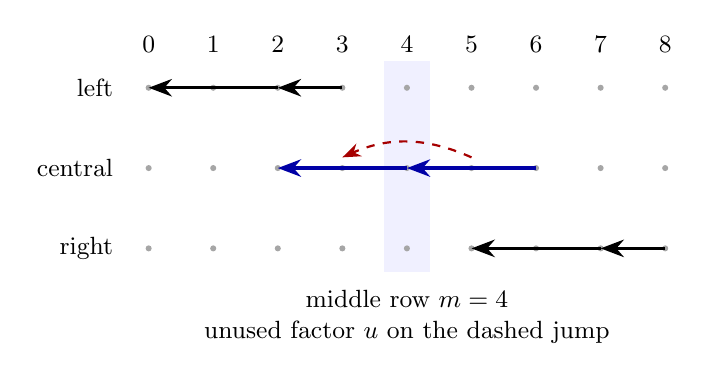
\begin{tikzpicture}[x=.82cm,y=.68cm,>=Stealth,font=\small]
 \fill[blue!6] (3.65,-.45) rectangle (4.35,3.5);
 \foreach \j in {0,...,8}{
  \node at (\j,3.8){\(\j\)};
  \foreach \h in {0,1.5,3}{\fill[black!35] (\j,\h) circle(1.1pt);}
 }
 \draw[->,very thick] (3,3)--(2,3);
 \draw[->,very thick] (2,3)--(0,3);
 \node[left] at (-.4,3){left};
 \draw[->,very thick,blue!65!black] (6,1.5)--(4,1.5);
 \draw[->,very thick,blue!65!black] (4,1.5)--(2,1.5);
 \draw[->,thick,dashed,red!65!black] (5,1.7) to[bend right=24] (3,1.7);
 \node[left] at (-.4,1.5){central};
 \draw[->,very thick] (8,0)--(7,0);
 \draw[->,very thick] (7,0)--(5,0);
 \node[left] at (-.4,0){right};
 \node[below,align=center] at (4,-.6){middle row \(m=4\)\\
           unused factor \(u\) on the dashed jump};
\end{tikzpicture}
\caption{The partition at the illustrative odd level \(N=9\).
A central path may visit row \(m\), or skip it by \(m+1\to m-1\).
The skipped row contributes its unused factor \(u\), retained in the
exact central polynomial even though it vanishes at \(u=0\).}
\label{lc:path-figure}
\end{figure}


\subsection{Cleared cofactors}
Let \(R_j(b;u)\) be the determinant obtained from the block of
\(\mathsf M\) on rows \(0,\ldots,j\) by replacing its last row with
\((1,b,\ldots,b^j)\). Its path expansion gives
\begin{equation}\label{lc:R-recurrence}
\begin{split}
 R_0&=1,\qquad R_{-1}=R_{-2}=0,\\
 R_j(b;u)&=b^j\prod_{r<j}\alpha_r+s_j^2A R_{j-1}(b;u)
                +s_js_{j-1}\alpha_{j-1}P R_{j-2}(b;u).
\end{split}
\end{equation}\aliascurrentequation{\label{sa:R}}
Equivalently, group the paths by their starting row:
\begin{equation}\label{sa:path}
 \begin{gathered}
 R_j=\sum_{i=0}^j b^i\prod_{r<i}\alpha_r K_{i,j},\qquad
 K_{i,i}=1,\quad K_{i,i-1}=0,\\
 K_{i,k}=s_k^2A K_{i,k-1}+s_ks_{k-1}\alpha_{k-1}P K_{i,k-2}.
 \end{gathered}
\end{equation}
The interval polynomial $K_{i,j}$ sums the paths between rows $i$ and $j$.
Both this formula and \eqref{lc:R-recurrence} are polynomial identities
when a diagonal factor vanishes.

The first term at \(j=0\) is the empty product one. Each \(R_j\)
has face degree \(j\) and spectral degree at most \(j\). Put
\[
 D_b=R_{m-1}(b;u),\qquad E_b=\alpha_{m-1}R_{m-2}(b;u),
\]
with \(E_b=0\) when \(m=1\). Subscripts \(b,c\) here denote substitution
of the middle variable, not differentiation.

\begin{lemma}[Exact central factors]\label{lc:central-factors}
At \(N=2m\),
\begin{equation}\label{lc:even-factor}
 \mathcal P_{\mathrm C}
 =s_m^2A D_bD_c+s_ms_{m-1}P(D_bE_c+E_bD_c).
\end{equation}\aliascurrentequation{\label{sa:even}}
At \(N=2m+1\), with \(G_b=R_m(b;u)\),
\begin{equation}\label{lc:odd-factor}
 \mathcal P_{\mathrm C}=G_bG_c+u s_m^2P D_bD_c.
\end{equation}\aliascurrentequation{\label{sa:odd}}
Both are polynomial identities for every \(u\).
\end{lemma}
\begin{proof}
An even central path crosses the cut exactly once, by \(m\to m-1\),
\(m+1\to m-1\), or \(m\to m-2\). Their weights give the three
terms. Reflection \(r\mapsto d-r\) identifies upper and lower
cofactors: \(a_{d-r}=a_r\), and the reflected step products agree.
At odd level, paths visiting \(m\) split there to give \(G_bG_c\).
A path skipping it has the unique jump \(m+1\to m-1\), with weight
\(s_{m+1}s_mP=s_m^2P\); its unused diagonal is \(u\).
This proves the second term without dividing by \(u\).
\end{proof}

The same reflection interchanges the left and right sectors and \(b,c\).
A one-step at \(r\) reflects to one at \(N-r\), with \(s_{N-r}=s_r\);
a two-step reflects to one at \(N+1-r\), with product \(s_{r-1}s_r\).
It therefore suffices to estimate the left sector.


\section{Exact nodal control of the central sector}\label{lc:nodal}
For face polynomials, \(F\coefle G\) means that every coefficient of
\(G-F\) is nonnegative real. The symbol \(\abscoef F\) replaces each
coefficient by its modulus. Recall that \(J=\lfloor(N-1)/2\rfloor\).
The \(J+1\) distinct physical nodes in the \(u\) coordinate are
\[
                         u_a=-a_a,\qquad 0\le a\le J.
\]
They include zero at odd level, but not at even level.

\begin{lemma}[Nodal positivity and comparison]\label{lc:nodal-positive}
For every \(0\le j,a\le J\),
\[
                    0\coefle R_j(b;u_a)\coefle R_j(b;0).
\]
\end{lemma}
\begin{proof}
If \(j\le a\), every diagonal factor used in \eqref{lc:R-recurrence}
lies between zero and its value at \(u=0\); induction proves the claim.
If \(j>a\), the inhomogeneous term vanishes after row \(a\).
Every surviving path must visit row \(a\), so
\[
                    R_j(b;u_a)=K_{a,j}(u_a)R_a(b;u_a),
\]
with $K_{a,j}$ defined in \eqref{sa:path}.
Normalize \(q_r=K_{a,a+r}/\prod_{v=a+1}^{a+r}s_v^2\).
For \(r\ge2\), \(j=a+r\le J\), product-to-sum gives
\[
 a_{j-1}-a_a=-s_{j+a}s_{j-a-1},\qquad
 s_js_{j-1}-s_{j+a}s_{j-a-1}=s_as_{a+1}.
\]
All the indicated sines are nonnegative. Thus
\begin{equation}\label{lc:tail-node}
 q_0=1,\quad q_1=x+y,\quad
 q_r=(x+y)q_{r-1}-\gamma_rxyq_{r-2},\qquad
 \gamma_r=1-\frac{s_as_{a+1}}{s_js_{j-1}}\in[0,1].
\end{equation}
The identity
\[
 q_r-xq_{r-1}
 =y(q_{r-1}-xq_{r-2})+(1-\gamma_r)xyq_{r-2}
\]
proves simultaneous coefficientwise positivity, starting from
\(q_0=1,q_1-xq_0=y\). Also \(q_r\coefle(x+y)^r\).
At \(u=0\), the interval continuant contains this all-one-step term
and other nonnegative terms. Hence \(K_{a,j}(u_a)\coefle K_{a,j}(0)\).
The product \(K_{a,j}(0)R_a(b;0)\) is the subset of paths in \(R_j(b;0)\)
whose start is at or below \(a\) and which visit \(a\). This proves
the assertion without assuming positivity of the signed recurrence.
\end{proof}

\begin{lemma}[Exact interpolation bound]\label{lc:interpolation}
An absolute constant \(C\) gives, for \(j\le J\),
\begin{equation}\label{lc:cofactor-comparison}
 \abscoef{R_j(b;u)}\coefle C(1+\log N)R_j(b;0),\qquad -4\le u\le0.
\end{equation}
\end{lemma}
\begin{proof}
Each face coefficient is a polynomial in \(u\) of degree at most
\(j\le J\). This interpolation is not applied to the degree-\(d\)
full resolvent. Use \(z=-1-u/2\) and
\(\phi_k=(2k+1)\pi/N\), \(0\le k<N\).
For a polynomial \(p(z)\) of degree at most \(J\), discrete Fourier
inversion gives
\[
 p(\cos t)=\frac1N\sum_{k=0}^{N-1}D_J(t-\phi_k)p(\cos\phi_k),
 \qquad D_J(v)=\sum_{\ell=-J}^Je^{i\ell v}.
\]
The difference of any two retained modes has magnitude less than \(N\),
so its grid average is a Kronecker delta. Pairing equal cosine nodes
gives ordinary interpolation, with the unpaired point \(-1\) at odd \(N\).
Since
\[
 |D_J(v)|\le\min(2J+1,|\sin(v/2)|^{-1}),
\]
the normalized sum of absolute kernel values on any translate of the
grid is at most \(C(1+\log N)\). The two nearest points cost a constant;
successive distances \(k/N\) cost at most \(C/k\). Pairing cannot
increase this bound. Apply it to each coefficient and use
Lemma~\ref{lc:nodal-positive}.
\end{proof}

\begin{proposition}[Central polynomial comparison]\label{lc:central-comparison}
For an absolute \(C\) and every \(N\ge3\),
\begin{equation}\label{lc:central-coefficientwise}
 \abscoef{\mathcal P_{\mathrm C}(u)}
 \coefle C(1+\log N)^2\mathcal P_{\mathrm C}(0),\qquad -4\le u\le0.
\end{equation}
\end{proposition}
\begin{proof}
Apply \eqref{lc:cofactor-comparison} to the exact central factors.
The scalar factors \(|u|,|a_{m-1}+u|\) are at most four.
At even \(N\ge4\),
\[
 D_b(0)\coefge s_{m-1}^2(x+y)R_{m-2}(b;0),\qquad (x+y)^2\coefge2xy.
\]
The sine is uniformly bounded below. Thus either mixed term
\(xyD_b(0)R_{m-2}(c;0)\) is bounded coefficientwise by a constant
times \((x+y)D_b(0)D_c(0)\), already present at zero.
At odd levels,
\[
 G_b(0)\coefge s_m^2(x+y)D_b(0),\qquad
 G_b(0)G_c(0)\coefge2s_m^4xyD_b(0)D_c(0).
\]
Here \(s_m\) is bounded below, including \(N=3\).
The skipped-middle term is therefore controlled as well.
\end{proof}


\section{A signed interval transfer estimate}\label{lc:transfer}
This section bounds the signed recurrence. It is not a Perron estimate
for its entrywise absolute value. Parametrize the real interval by
\[
 \sigma=-2\cos(2\pi\delta),\qquad u=-4\sin^2(\pi\delta),
                    \qquad0\le\delta\le\tfrac12.
\]
For positive outer sum \(A=x+y\) and \(P=xy\ge0\), define
\begin{equation}\label{lc:continuous-coefficients}
\begin{aligned}
 a_\delta(t)&=4(\cos^2(\pi t)-\sin^2(\pi\delta)),\\
 \rho_\delta(t)&=A\sin(\pi t)+
   \sqrt{(x-y)^2\sin^2(\pi t)+4P\cos^2(\pi\delta)},\\
 \lambda_\delta(t)&=2\sin(\pi t)\rho_\delta(t).
\end{aligned}
\end{equation}
On each compact set of allowed moduli,
\begin{equation}\label{lc:endpoint-size}
 ct\le\rho_\delta(t)\le C,\qquad ct^2\le\lambda_\delta(t)\le C,
                          \qquad0<t\le\tfrac12,
\end{equation}
uniformly in \(\delta\).

\begin{lemma}[Uniform signed transfer]\label{lc:slow-transfer}
For every \(\varepsilon>0\), all sufficiently large \(N\) satisfy
\begin{equation}\label{lc:transfer-estimate}
 |K_{i,j}|\le
 \exp\left\{N\int_{i/N}^{j/N}\log\lambda_\delta(t)\,dt+\varepsilon N\right\},
                      \qquad0\le i\le j\le m.
\end{equation}
The threshold is uniform in endpoints, real spectral parameter,
and each fixed compact set of allowed moduli.
\end{lemma}
\begin{proof}
Normalize \(L_{i,j}=K_{i,j}/\prod_{r=i+1}^js_r\). Its step matrix is
\[
 T_h(t,\delta)=
 \begin{pmatrix}
 2A\sin(\pi t)&4P[\cos^2(\pi(t-h/2))-\sin^2(\pi\delta)]\\1&0
 \end{pmatrix},\quad h=N^{-1},\quad t=jh.
\]
The limiting matrix has real eigenvalues
\[
 A\sin(\pi t)\ \pm\
       \sqrt{(x-y)^2\sin^2(\pi t)+4P\cos^2(\pi\delta)}.
\]
Its spectral radius is \(\rho_\delta(t)\), including coincident roots.
Use the Euclidean operator norm. Fix \(\eta>0\) and restrict to
\(t\in[\eta,1/2]\), where
\(\rho_\delta(t)\ge c_\eta>0\). Cayley--Hamilton gives uniformly
\begin{equation}\label{lc:constant-power}
                    \|T^k\|\le C_\eta(k+1)\rho(T)^k .
\end{equation}
For distinct eigenvalues the power divided difference is a sum of
\(k\) terms, each bounded by \(\rho^{k-1}\). The polynomial identity
extends to coincident eigenvalues by its derivative value. Bounded
entries and the positive lower bound on \(\rho\) give \(C_\eta\).
No eigenbasis or its condition number is used.

Choose a fixed block length \(k\) for which
\(\log(2C_\eta(k+1))/k\) is smaller than a prescribed error.
Within a block, the exact matrices differ from its first limiting
matrix by \(O_k(N^{-1})\). Expanding the finite product one factor
at a time bounds its difference from \(T^k\) by the same order.
For large \(N\) this is at most \(C_\eta(k+1)\rho^k\).
Multiplying block bounds and using uniform continuity of \(\log\rho\)
gives its integral plus the prescribed error. Incomplete blocks have
at most \(2k\) factors and cost \(o(N)\), uniformly in the endpoints.

For \(0<t<\eta\), bounded entries cost at most \(C^{\eta N+O(1)}\).
The omitted logarithmic integral has absolute value at most
\(C\eta\log(2/\eta)\), by \eqref{lc:endpoint-size}.
The exact scalar factors \(s_r\) have the same integrable endpoint
bound, and their logarithmic Riemann sums converge uniformly over
subintervals. Choose \(\eta\) first, then the fixed block length,
and finally \(N\). Restoring these factors proves the estimate.
If a perturbation of the reference matrices is wanted, it must be
chosen after the block length; a sufficiently small fixed perturbation
then fits the same finite-product error. No complex perturbation is
needed for the theorem here.
\end{proof}

\subsection{Unused spectral rows}
The exact diagonals are \(\alpha_r=a_\delta((r+1/2)/N)\).
Uniformly in \(\delta\) and interval endpoints,
\begin{equation}\label{lc:riemann}
 \sum_{r=l}^{k-1}\log|\alpha_r|
 \le N\int_{l/N}^{k/N}\log|a_\delta(t)|\,dt+o(N).
\end{equation}
A sampled zero makes the left side \(-\infty\), which causes no
upper-bound problem. This convention describes a zero product;
no finite division by it is made.

For a proof, truncate the logarithm from below at \(-M\).
The truncated function is jointly continuous, so its Riemann sums
converge uniformly. The factorization
\[
 a_\delta(t)=4\cos(\pi(t+\delta))\cos(\pi(t-\delta))
\]
shows that \(\{|a_\delta|<r\}\) has length at most \(C\sqrt r\),
uniformly in \(\delta\). Integrating this distribution bounds the
omitted logarithmic tails uniformly by a quantity tending to zero
as \(M\to\infty\). The argument applies to every subinterval.

There is also the exact complete-prefix identity
\begin{equation}\label{lc:prefix-zero}
                   \int_0^{1/2}\log|a_\delta(t)|\,dt=0 .
\end{equation}
Shift the two cosine integrals and use the reflection and period
of \(\log|2\cos(\pi t)|\). Together they have the integral of a full
period, which is zero. Integrability includes \(\delta=0,1/2\).
We use this identity only after both actual unused products have
been bounded separately.


\section{The normalized triangle action}\label{lc:action}
For \(b>0\), define
\begin{equation}\label{lc:F}
 F_b(\mu,\delta)=\mu\log b+
 \int_0^\mu\log|a_\delta(t)|\,dt+
 \int_\mu^{1/2}\log\lambda_\delta(t)\,dt .
\end{equation}
When \(b=0\), only \(\mu=0\) is allowed. Use the exact starting-row decomposition \eqref{sa:path}.
Lemma~\ref{lc:slow-transfer}, \eqref{lc:riemann}, and at most \(N+1\)
starts give, for \(n=N/2+O(1)\) and \(n\le m\),
\begin{equation}\label{lc:cofactor-rate}
 |R_n(b;u)|\le
 \exp\left\{N\left[\max_{0\le\mu\le1/2}F_b(\mu,\delta)
                                      +\varepsilon\right]\right\}
\end{equation}
uniformly for large \(N\). Replacing \(n/N\) by \(1/2\) costs \(o(N)\),
since \(\lambda_\delta\) is uniformly positive at \(1/2\).

For \(0\le\delta<1/2\), put \(s=\sin(\pi\delta)\), \(k=\cos(\pi\delta)\),
and
\[
 T_b=\sqrt{bA+P+b^2s^2},\qquad
 \mathcal D=A^2-4Ps^2,\qquad
 \mathcal E_b=A+2bs^2+2sT_b.
\]
These scalar symbols are distinct from the finite cofactors \(D_b,E_b\).
The stationary point before the sign change \(t_c=1/2-\delta\) is
\begin{equation}\label{lc:mu}
 \mu_b=\frac1\pi\arctan\frac{bk}{T_b},\qquad
 \sin^2(\pi\mu_b)=\frac{k^2b^2}{(b+x)(b+y)}.
\end{equation}
For \(b=0\) set \(\mu_b=0\), and write
\(Q_b(\delta)=F_b(\mu_b,\delta)\).

\begin{lemma}[Calibration and spectral derivative]\label{lc:action-identity}
For the allowed nonnegative weights,
\begin{equation}\label{lc:calibration}
                       Q_b(0)=\mathcal Q(x,b,y).
\end{equation}
For \(0<\delta<1/2\),
\begin{equation}\label{lc:action-derivative}
             Q_b'(\delta)=-\log(\mathcal E_b/\sqrt{\mathcal D})\le0.
\end{equation}
If \(b=P=0\), the action is the constant \(\frac12\log A\).
The endpoint and zero-weight cases follow from the exact sole-start
or one-step formulas and their continuous limits.
\end{lemma}
\begin{proof}
The stationary equation is
\(b\,a_\delta(\mu)=\lambda_\delta(\mu)\) where \(a_\delta>0\).
Squaring its positive sides gives \eqref{lc:mu}.

First fix the constant in \eqref{lc:calibration}. For \(0<a<1/2\),
\[
 e'(a)=\log\cot(\pi a),\qquad
 e''(a)=-\frac{\pi}{\sin(\pi a)\cos(\pi a)}<0.
\]
At positive weights the entropy maximizer is unique and has loads
\[
 a_w=\frac1\pi\arctan\frac{w}{\sqrt{xb+xy+by}},
                          \qquad w=x,b,y .
\]
The tangent addition identity makes their sum \(1/2\), and the
three constrained derivatives are equal. Hence the derivative
of \(\mathcal Q(x,b,y)\) with respect to \(\log b\) is
\(a_b=\mu_b|_{\delta=0}\). The envelope rule gives the same
derivative for \(F_b(\mu_b,0)\), so their difference is independent
of \(b>0\). As \(b\to\infty\), both minus \(\frac12\log b\)
tend to zero. For the entropy this follows also directly from the
displayed loads: the other loads and their entropy terms tend to zero,
and their products with \(\log b\) vanish. For the integral,
\(1/2-\mu_b=O(b^{-1/2})\), the full prefix integral is zero,
and the remaining logarithmic tails vanish.
This proves equality without a geometric normalization.
Zero weights follow by continuity on the constrained faces of
the load simplex and by the dominated logarithmic integrals.

For the derivative, \(\partial_{\log b}Q_b=\mu_b\), and
direct differentiation gives
\[
 \partial_\delta\mu_b=-\frac{bs}{T_b},\qquad
 \partial_{\log b}\log(\mathcal E_b/\sqrt{\mathcal D})
                                      =\frac{bs}{T_b}.
\]
Thus \(Q_b'+\log(\mathcal E_b/\sqrt{\mathcal D})\) is independent
of \(b\). Determine it at \(b=0\), retaining the integration constant.
For \(P>0\), set \(\lambda=2\sqrt P/A\in(0,1]\).
Differentiating the sole-start integral and putting
\(\vartheta=\pi t\) gives
\[
 Q_0'=-\lambda^2sk\int_0^{\pi/2}
 \frac{d\vartheta}{W(\vartheta)(\sin\vartheta+W(\vartheta))},
 \quad W(\vartheta)=
       \sqrt{(1-\lambda^2)\sin^2\vartheta+\lambda^2k^2}.
\]
Rationalization and \(z=\cos\vartheta\) turn this into
\[
 -sk\int_0^1\left\{\frac1{\sqrt{1-z^2}}-
 \frac1{\sqrt{1-\lambda^2s^2-(1-\lambda^2)z^2}}\right\}
                                  \frac{dz}{z^2-s^2}.
\]
The apparent pole at \(z=s\) is removable. For either term,
\(B-Cs^2=k^2\), and differentiation verifies
\[
 \int\frac{dz}{(z^2-s^2)\sqrt{B-Cz^2}}
 =\frac1{2sk}\log\left|
     \frac{kz/\sqrt{B-Cz^2}-s}{kz/\sqrt{B-Cz^2}+s}\right|.
\]
Subtract the antiderivatives before evaluating. Their singularities
at \(z=s\) cancel. At zero both are zero; at one the first tends to
zero and the second gives the finite remaining term. The result is
\[
 Q_0'=-\operatorname{artanh}(\lambda s)
 =-\log\frac{A+2s\sqrt P}{\sqrt{A^2-4Ps^2}} .
\]
This proves \eqref{lc:action-derivative} for all \(b\ge0\).
When \(P=0\), the exact tail root is \(4A\sin^2(\pi t)\);
direct differentiation gives the same formula. It also follows by
dominated convergence as \(P\downarrow0\).
If \(b=P=0\), the integral is \(\frac12\log A\).
Finally \(\mathcal E_b\ge\sqrt{\mathcal D}>0\) in the open interval.
The possible singularity at \(x=y,\delta=1/2\) is logarithmic and
integrable.
\end{proof}

\begin{lemma}[The cofactor maximum]\label{lc:cofactor-max}
For \(b>0\),
\[
 \max_{0\le\mu\le1/2}F_b(\mu,\delta)
                =\max\{Q_b(\delta),\tfrac12\log b\}.
\]
For \(b=0\), the sole value is \(Q_0(\delta)\).
\end{lemma}
\begin{proof}
At a regular point, \(\partial_\mu F_b=\log(b|a_\delta|/\lambda_\delta)\).
Writing \(w=k^2/\sin^2(\pi\mu)\), the ratio is
\[
                  \frac{2b|w-1|}{A+\sqrt{(x-y)^2+4Pw}} .
\]
Before \(t_c\), \(w\) decreases from infinity to one and this ratio
strictly decreases from infinity to zero. To check its monotonicity
for \(w>1\), the positive derivative numerator after cancellation is
\[
             A+\frac{(x-y)^2+2Pw+2P}{\sqrt{(x-y)^2+4Pw}} .
\]
The case \(P=0\) is immediate. Thus the unique maximum there is
\(\mu_b\). After \(t_c\) the ratio increases with \(\mu\), so
every critical point is a minimum. The last endpoint has value
\(\frac12\log b\) by \eqref{lc:prefix-zero}; the first is below
the pre-sign-change maximum.
At \(\delta=1/2\), the ratio is the constant \(b/\max(x,y)\),
and the endpoint values prove the assertion. The continuous limit is
\(Q_b(1/2)=\frac12\log\max(x,y)\).
\end{proof}

At \(\delta=0\), these lemmas and
\(\mathcal Q(x,b,y)\ge\frac12\log b\) imply
\[
 R_{N/2+O(1)}(b;0)
                  \le\exp\{N(\mathcal Q(x,b,y)+\varepsilon)\}.
\]
Use this in the exact central factorization at zero. The scalar
coefficients and face monomials are bounded on each fixed compact.
Proposition~\ref{lc:central-comparison} then proves the central
part of Theorem~\ref{lc:main}, including arbitrary face phases.


\section{The one-sided envelope with both unused products}\label{lc:left}
For \(0\le i\le j<m\), the exact left summand is
\begin{equation}\label{lc:left-summand}
 A_{\rm rest}(u)b^ic^{d-j}
       \left(\prod_{r<i}\alpha_r\right)
       \left(\prod_{j<r<m}\alpha_r\right)K_{i,j}(u),
\end{equation}
where \(A_{\rm rest}=\prod_{r=m}^d\alpha_r\) is the whole omitted
upper-half product. On the real interval it has no positive
exponential cost. At \(N=2m\),
\[
 A_{\rm rest}(u)=2(-1)^mT_m(\sigma/2),\qquad |A_{\rm rest}|\le2.
\]
Its roots and leading coefficient prove the identity.
At \(N=2m+1\), it is, up to sign, \((\sigma+2)P_m(\sigma)\), where
\[
 P_m(2\cos t)=\frac{\cos((m+1/2)t)}{\cos(t/2)}.
\]
The quotient is a finite alternating sum of \(m\) paired exponentials
and one constant, so \(|P_m|\le2m+1=N\).
Hence \(|A_{\rm rest}|\le4N\), including the removable endpoint.
These are the original unused products, not auxiliary normalizations.

For \(b,c>0\), apply the transfer and Riemann estimates separately
to the two outside products in \eqref{lc:left-summand}. Only then
use \eqref{lc:prefix-zero}. With \(\mu=i/N,\nu=j/N\), the upper
action becomes
\begin{equation}\label{lc:left-action}
\begin{split}
 F_{\mathrm L}(\mu,\nu,\delta)
 &=\mu\log b+(1-\nu)\log c+
                   \int_\mu^\nu\log L_\delta(t)\,dt,\\
 L_\delta(t)&=\frac{\lambda_\delta(t)}{|a_\delta(t)|},
                      \qquad0\le\mu\le\nu\le\tfrac12.
\end{split}
\end{equation}
This quotient is only continuum notation. No finite division by
\(\alpha_r\) occurred. Moving an endpoint by \(O(N^{-1})\) changes
the integrals by \(o(1)\) uniformly, by logarithmic integrability.
There are at most \(N^2\) pairs \((i,j)\), contributing only \(o(N)\).
If \(b=0\), the finite sum has only \(i=0\), so only \(\mu=0\)
is allowed. If \(c=0\), the left polynomial vanishes because
\(d-j\ge\lfloor N/2\rfloor>0\).

\begin{proposition}[Exact continuum envelope]\label{lc:left-maximum}
For \(c>0,b\ge0\),
\begin{equation}\label{lc:left-envelope}
 \sup_{\substack{0\le\delta\le1/2\\0\le\mu\le\nu\le1/2}}
 F_{\mathrm L}(\mu,\nu,\delta)
       =\max\{\log c,\mathcal Q(x,b,y)+\tfrac12\log c\}.
\end{equation}
For \(b=0\) restrict the left side to \(\mu=0\).
This is an equality of continuum upper envelopes, not a lower
bound for an oscillatory finite polynomial.
\end{proposition}
\begin{proof}
First assume \(b>0\), \(0<\delta<1/2\), and set
\(z=\sin^2(\pi\delta)\), \(\mathcal D=A^2-4Pz\).
The ratio calculation in Lemma~\ref{lc:cofactor-max} shows that
\(L_\delta\) increases from zero to infinity before \(t_c\) and
decreases from infinity to
\[
                         L_{\rm end}=\frac{A+\sqrt{\mathcal D}}{2z}
\]
afterward. The endpoint derivatives are
\[
 \partial_\mu F_{\mathrm L}=\log b-\log L_\delta(\mu),\qquad
 \partial_\nu F_{\mathrm L}=\log L_\delta(\nu)-\log c.
\]
A stationary \(\nu<t_c\) is a minimum, and a stationary \(\mu>t_c\)
is a minimum. The logarithmic singularity creates no maximum:
the derivative in \(\nu\) is positive on both sides near \(t_c\),
and that in \(\mu\) is negative. The boundary \(\mu=0\) is excluded
for \(b>0,\nu>0\) by its positive initial derivative.
Apart from the diagonal \(\mu=\nu\), the possible maxima therefore
have \(\mu=\mu_b\) and either \(\nu=1/2\) or a stationary
\(\nu_c>t_c\).

The diagonal contributes at most
\(\max(\log c,\frac12\log b+\frac12\log c)\).
The terminal value is \(Q_b(\delta)+\frac12\log c\), because the
complete prefix integral is zero. Both are bounded by the proposed
answer, using Lemma~\ref{lc:action-identity} and
\(\mathcal Q(x,b,y)\ge\frac12\log b\).

A post-change stationary endpoint exists precisely when
\(c\ge L_{\rm end}\). If \(c\le\max(x,y)\), this never occurs
in the open interval. Otherwise it begins at \(\delta_c\), where
\begin{equation}\label{lc:nu-c}
 \sin^2(\pi\delta_c)=\frac Ac-\frac P{c^2},\qquad
 \sin^2(\pi\nu_c)
       =\frac{c^2\cos^2(\pi\delta)}{(c-x)(c-y)}.
\end{equation}
At entry \(\nu_c=1/2\), and afterward \(t_c<\nu_c<1/2\).
Define
\[
 J_c(\delta)=\nu_c\log c+
 \int_0^{\nu_c}\log|a_\delta(t)|\,dt+
 \int_{\nu_c}^{1/2}\log\lambda_\delta(t)\,dt.
\]
The straddling value is exactly
\begin{equation}\label{lc:straddling}
                  S_{\mathrm L}=Q_b(\delta)+\log c-J_c(\delta).
\end{equation}
Subtracting the displayed integrals and using
\eqref{lc:prefix-zero} proves this with no additive constant.

Put \(T_c^-=\sqrt{c^2z-cA+P}\) and
\(\mathcal H_c=2cz-A+2\sqrt z\,T_c^-\). On the strict branch,
\begin{equation}\label{lc:J-derivative}
                  J_c'=-\log(\mathcal H_c/\sqrt{\mathcal D}).
\end{equation}
Here is a normalization proof. The stationary envelope rule gives
\(\partial_{\log c}J_c=\nu_c\), while direct differentiation gives
\[
 \partial_\delta\nu_c=-\frac{c\sin(\pi\delta)}{T_c^-},\qquad
 \partial_{\log c}\log\mathcal H_c=
                         \frac{c\sin(\pi\delta)}{T_c^-}.
\]
Thus the difference in \eqref{lc:J-derivative} is independent of
\(c\) for each \(\delta\). At \(c\downarrow L_{\rm end}\), one has
\(\nu_c\to1/2\), \(T_c^-\to0\), and \(\mathcal H_c\to\sqrt{\mathcal D}\).
The complete prefix integral has zero derivative. The remaining
tail shrinks where \(a_\delta(1/2)\ne0\), so \(J_c'\to0\).
This fixes the constant. To justify differentiation despite the
interior logarithmic zero, write \(\ell(t)=\log|2\cos(\pi t)|\).
At fixed \(\nu>t_c\), the prefix integral is
\[
 \int_\delta^{\nu+\delta}\ell(t)\,dt+
 \int_{-\delta}^{\nu-\delta}\ell(t)\,dt.
\]
Its derivative is
\(\ell(\nu+\delta)-\ell(\nu-\delta)\); the two terms at
\(\pm\delta\) cancel. The moving zero lies strictly inside the
integration interval, while all its endpoints are regular.
Thus this primitive differentiates normally on the strict branch.
At \(\nu=1/2\) its derivative is zero. The tail integral has
smooth integrand there, so the stated branch-entry limit follows.

It follows that \(S_{\mathrm L}'=\log(\mathcal H_c/\mathcal E_b)\).
Both positive quantities are larger roots with the same product
\(\mathcal D\):
\[
\begin{aligned}
 \mathcal E_b&=C_b+\sqrt{C_b^2-\mathcal D},&C_b&=A+2bz,\\
 \mathcal H_c&=C_c+\sqrt{C_c^2-\mathcal D},&C_c&=2cz-A.
\end{aligned}
\]
Both \(C_b,C_c\ge\sqrt{\mathcal D}\). The larger-root function is
increasing, and hence
\[
             \operatorname{sign}S_{\mathrm L}'
                      =\operatorname{sign}((c-b)z-A).
\]
As \(z\) increases, this sign can pass only from negative to positive.
There is no interior spectral maximum. At branch entry the value
is the terminal value already bounded. At \(\delta\to1/2\), both
\(\mu_b,\nu_c\to0\), and logarithmic integrability gives
\(S_{\mathrm L}\to\log c\). The upper bound follows.

The continuum candidates are attained: \(\mu=\nu=0\) gives \(\log c\),
and \(\delta=0,\nu=1/2,\mu=\mu_b\) gives
\(\mathcal Q(x,b,y)+\frac12\log c\).
For \(b=0\), use its sole start or the continuous limiting formulas.
For \(P=0\), the exact one-step root gives the same identities
without division by \(P\). The exceptional \(\mathcal D=0\) occurs
only at \(x=y,\delta=1/2\), where the computed continuous endpoint
values apply.
\end{proof}


\section{Face phases and the last spectral cap}\label{lc:phases}
To use the signed real transfer at arbitrary face phases, we need
positivity of the interval continuant itself, rather than positivity
of its recurrence coefficients.

\begin{lemma}[Continuous real positivity of interval tails]\label{lc:tail-positive}
For \(0\le i\le j\le m\) and
\(0\le\delta\le1/2-1/(2N)\), \(K_{i,j}\) has nonnegative coefficients
in \(x,y\). Consequently
\[
 |K_{i,j}(X_0,Y_0;\delta)|
                 \le K_{i,j}(|X_0|,|Y_0|;\delta).
\]
\end{lemma}
\begin{proof}
Set \(U_r=K_{i,i+r}/\prod_{v=i+1}^{i+r}s_v^2\).
Then \(U_0=1,U_1=x+y\), and for \(r\ge2\), \(j=i+r\),
\[
 U_r=(x+y)U_{r-1}+\beta_jxyU_{r-2},\qquad
                       \beta_j=\frac{\alpha_{j-1}}{s_js_{j-1}}.
\]
The recurrence starts at its second step, so it never divides by \(s_0\).
Product-to-sum gives the row-independent identity
\[
 \alpha_{j-1}+s_js_{j-1}
             =4\cos^2(\pi\delta)-4\sin^2(\theta/2)\ge0.
\]
Thus \(1+\beta_j\ge0\), even if \(\beta_j<0\). Simultaneous induction
using
\[
 U_r-xU_{r-1}
   =y(U_{r-1}-xU_{r-2})+(1+\beta_j)xyU_{r-2}
\]
and \(U_0=1,U_1-xU_0=y\) proves positivity. Taking moduli in a
polynomial with nonnegative coefficients proves the last assertion.
\end{proof}

In \eqref{lc:left-summand}, take absolute values of the middle
monomials and of the scalar unused products. The lemma then permits
the positive outer moduli in the \emph{same signed} continuant.
Thus Proposition~\ref{lc:left-maximum} bounds every face phase
uniformly for
\[
                       -2\le\sigma\le b_N:=2\cos(\pi/N).
\]
No positivity of the full numerator, or comparison of its unused
products to their endpoint values, has been asserted.

For the small remaining interval, let \(p\) be any complex polynomial
of degree at most \(d\), bounded by \(M\) on \([-2,b_N]\).
The affine coordinate of \(\sigma=2\) relative to this interval is
\(z_N=(6-b_N)/(b_N+2)\).
For a degree-\(d\) polynomial \(r\), the function
\(w^{-d}r((w+w^{-1})/2)\) is holomorphic outside the unit disk and
at infinity. On its boundary it is bounded by \(\|r\|_{[-1,1]}\).
The maximum principle on the reciprocal disk gives
\[
 |r(z)|\le\|r\|_{[-1,1]}\exp(d\,\operatorname{arcosh}z),\qquad z\ge1.
\]
Complex coefficients cause no change. As \(z_N=1+O(N^{-2})\),
uniformly for \(N\ge3\),
\begin{equation}\label{lc:last-cap}
 \sup_{-2\le\sigma\le2}|p(\sigma)|
      \le M\exp(d\,\operatorname{arcosh}z_N)\le C M.
\end{equation}
For each fixed face-phase tuple the actual left polynomial has
spectral degree at most \(d\). Apply \eqref{lc:last-cap} before
taking the supremum of those phases. The constant is independent
of them. This proves the left assertion of Theorem~\ref{lc:main}.
Row reflection proves the right assertion. The central assertion
was proved in Section~\ref{lc:action}. Every compact estimate
respects the declared zero pattern, completing the theorem.


\section{Shared face coefficients}\label{cs:shared}
A fixed finite collection of boxes may be assigned genuine labels
\(s_e\), with every occurrence of each face variable identified.
Keep designated zero faces exactly zero. Let \(t_f\) be the ordinary
coefficient targets, and choose a single positive radius \(\rho_f\)
for each remaining face. Require that the sum of the two outer moduli
is positive in every box; a zero pattern killing both outer variables
is outside Theorem~\ref{lc:main}. Cauchy's coefficient formula gives
\[
 \left|[L^t]\prod_eH_{V,s_e}(L;\sigma_e)\right|
 \le\prod_f\rho_f^{-t_f}
       \sup_{|L_f|=\rho_f}\prod_e|H_{V,s_e}(L;\sigma_e)|.
\]
Theorem~\ref{lc:main} applies at this shared radius vector. If
\(t_f/N\to\tau_f\), the uniform real-cube upper rate is at most
\[
                      \sum_eA_{s_e}(\rho)-\sum_f\tau_f\log\rho_f .
\]
The number of boxes is fixed before \(N\) grows, so their errors sum
to \(o(N)\). For finitely many sector strings, take the maximum of
these sums before bounding their finite sum. This keeps correlations
between genuine labels; no Cartesian enlargement is needed.

This argument gives an upper bound for each prescribed sector choice.
The coefficientwise comparison \eqref{lc:central-coefficientwise} applies
to the central sector. The one-sided estimates remain bounds on values;
we have not proved coefficientwise domination for them.

\subsection{The marked triangulation and its central coefficient}
Let $\mathcal T$ be a finite simple oriented triangulation of the sphere.
A perfect matching of its dual pairs its triangles across $R$ edges.
Its $R+2$ vertices are called faces, following their role in the original
diagram. Choose a nonmatching edge $uv$ as the mark. The two face
variables $L_u,L_v$ are set to zero; the remaining $R$ variables are
ordinary. The order at a matched pair is $(x,b,c,y)$: its triangles
are $(x,b,y)$ and $(x,c,y)$, with their induced opposite orientations
along the matching edge $xy$. Repeated occurrences of a face always
denote the same variable.
In particular $x+y>0$ on the positive ordinary radii of every pair:
otherwise its matching edge would be the unique edge $uv$, which is
the nonmatching mark. Each pair also has a nonmonomial triangle.
If one outer face is protected, only one other zero remains, so at
least one middle is positive; if both outers are positive, both
triangles are nonmonomial.

Use the operator and face polynomial of Section~\ref{lc:source}, with
$d=N-1$ and $J=\lfloor d/2\rfloor$. The central sector is equivalently
the set of paths with $i\le J$ and $d-j\le J$. At each matched edge
we select this sector of the same divided difference $V_N$.

Put $\sigma_e=-2\cos(2\pi\delta_e)$ and define the raw central coefficient
\begin{equation}\label{sa:coefficient}
 C_N(\delta)=
 \left[\prod_{f\ne u,v}L_f^d\right]
 \left.\prod_{e=1}^R H_{V,\mathrm C}
       (L_{x_e},L_{b_e},L_{c_e},L_{y_e};\sigma_e)
                  \right|_{L_u=L_v=0}.
\end{equation}
This definition includes its sign $(-1)^{dR}$. Its identification as a
contribution to the original marked evaluation, with cups, caps and
framing still present, is the exact diagram theorem
\cite[Theorem 9.1 and Corollary 9.2]{FinitePaper}. The coefficient itself is
the object of the present analytic theorem.

\begin{figure}[t]
\centering
% Native TikZ source. Incidence drawing, not a circle packing.
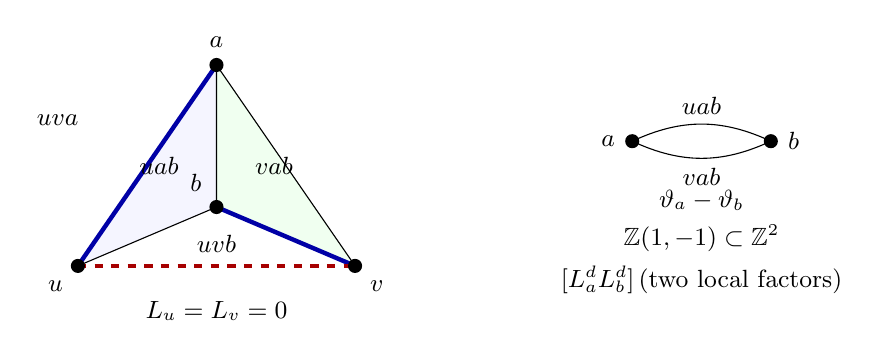
\begin{tikzpicture}[scale=.88, every node/.style={font=\small},
  vertex/.style={circle,fill=black,inner sep=1.8pt},
  matching/.style={draw=blue!65!black,line width=1.6pt},
  marked/.style={draw=red!65!black,dashed,line width=1.2pt}]
  \coordinate (u) at (-2,0);
  \coordinate (v) at (2,0);
  \coordinate (a) at (0,2.9);
  \coordinate (b) at (0,.85);
  \fill[blue!4] (u)--(a)--(b)--cycle;
  \fill[green!6] (v)--(a)--(b)--cycle;
  \draw[matching] (u)--(a);
  \draw[matching] (v)--(b);
  \draw[marked] (u)--(v);
  \draw (u)--(b)--(a)--(v);
  \node[vertex,label=below left:$u$] at (u) {};
  \node[vertex,label=below right:$v$] at (v) {};
  \node[vertex,label=above:$a$] at (a) {};
  \node[vertex,label=above left:$b$] at (b) {};
  \node at (-.83,1.45) {$uab$};
  \node at (.83,1.45) {$vab$};
  \node at (0,.32) {$uvb$};
  \node[anchor=east] at (-1.85,2.1) {$uva$};
  \node at (0,-.65) {$L_u=L_v=0$};
  \begin{scope}[xshift=7cm]
    \coordinate (aa) at (-1,1.8);
    \coordinate (bb) at (1,1.8);
    \draw (aa) to[bend left=25] node[above] {$uab$} (bb);
    \draw (aa) to[bend right=25] node[below] {$vab$} (bb);
    \node[vertex,label=left:$a$] at (aa) {};
    \node[vertex,label=right:$b$] at (bb) {};
    \node[align=center] at (0,.65)
      {$\vartheta_a-\vartheta_b$\\[3pt]$\mathbb Z(1,-1)\subset\mathbb Z^2$};
    \node at (0,-.2) {$[L_a^dL_b^d]\,(\text{two local factors})$};
  \end{scope}
\end{tikzpicture}

\caption{A combinatorial tetrahedral sphere and its ordinary phase graph.
The vertices $u,v,a,b$ name shared face variables. The marked edge $uv$
(red, dashed) sets $L_u=L_v=0$; the two blue matching edges are $ua$
and $vb$. The outer face of the planar drawing is the triangle $uva$.
The two triangles with two ordinary vertices, $uab$ and $vab$, compare the same
ordinary phases $\vartheta_a,\vartheta_b$, giving two copies of the
primitive difference row $(1,-1)$. Their coefficients add in the
Hessian, while the quotient angular measure remains
$d\vartheta_b/(2\pi)$ after $\vartheta_a=0$. The coefficient target is
$L_a^dL_b^d$, with each variable shared by the two local factors.
The edge lengths in this combinatorial drawing do not prescribe the radii
in the variational problem.}
\label{sa:shared-figure}
\end{figure}

Here is the sole positive-radius input. It can be supplied by the
complete packing of the marked triangulation, but is stated analytically
so that the theorem can be used without a geometric normalization.
Use the triangle function $\mathcal Q$ defined in \eqref{lc:entropy},
with every protected face kept exactly zero.
Choose positive ordinary radii $\rho_f$ such that
\begin{equation}\label{sa:stationarity}
 \mathcal F(L)=\sum_{e=1}^R
     \{\calQ(x_e,b_e,y_e)+\calQ(x_e,c_e,y_e)\}
                         -\sum_{f\ne u,v}\log L_f
 \quad\text{is stationary at }L=\rho
\end{equation}
modulo common scale. Set $\Phi=\mathcal F(\rho)$.
Zeros remain exactly zero. The diagram and radii are fixed before $N$
tends to infinity.

\begin{theorem}[Asymptotic of the shared central coefficient]\label{sa:main}
Under these hypotheses there is a fixed complex polydisk about zero
and, for all sufficiently large $N$, holomorphic functions $A_N$ and
holomorphic $(R-1)$-by-$(R-1)$ matrices $H_N$ on it such that
\begin{equation}\label{sa:H1}
 C_N(\delta)=
 \frac{(-1)^{dR}N^{2R}e^{NA_N(\delta)}}
 {(2\pi N)^{(R-1)/2}\sqrt{\det H_N(\delta)}}
                         (1+O(N^{-1})).
\end{equation}
The relative error is holomorphic and uniform on smaller closed
polydisks. The square root continues the positive face Hessian at zero.
The actions are separately even and real on the real chart, and
$A_N\to A_0$, $H_N\to H_0$ locally uniformly with every fixed derivative.
The face Hessian $H_0(0)$ is positive definite. Moreover
\begin{equation}\label{sa:hessian}
 \begin{aligned}
 A_0(0)&=\Phi,\qquad A_0''(0)=-2\operatorname{diag}(\kappa_e),\\
 \kappa_e&=\frac{\pi\bigl(\sqrt{b_e(x_e+y_e)+x_ey_e}
                    +\sqrt{c_e(x_e+y_e)+x_ey_e}\bigr)}
                    {x_e+y_e}>0.
 \end{aligned}
\end{equation}
All face values in the last expression are at $\rho$.

For every $0<\eta<1/2$ there are $\gamma_\eta,\tau_\eta>0$ such that,
for all sufficiently large integer levels,
\begin{equation}\label{sa:H2}
 |C_N(x+\ii y)|\le e^{N(\Phi-\gamma_\eta)}
 \quad(x\in[-1/2,1/2]^R,\ \max_e|x_e|\ge\eta,
                       \ \max_e|y_e|\le\tau_\eta).
\end{equation}
Fixed derivatives have the corresponding bounds on smaller domains.
There is no prime-level restriction and no change of normalization
between even and odd levels.
\end{theorem}

We define the finite actions directly from the actual local polynomial.
They are not asserted to equal a separately constructed approximate
fold interpolation. In particular no value-only interpolation is
differentiated to obtain a normal.


\section{Positive matrices at the finite spectral nodes}\label{sa:finite}
We use the cofactors $R_j$ and interval polynomials $K_{i,j}$ of
\eqref{lc:R-recurrence}--\eqref{sa:path}. Throughout the remaining
sections, $u(\delta)=-4\sin^2(\pi\delta)$ denotes the spectral coordinate;
it is distinct from the protected vertex $u$ of the triangulation.
We also write $P_{\mathrm C}=\mathcal P_{\mathrm C}=(-1)^dH_{V,\mathrm C}$.
The central factorizations \eqref{lc:even-factor}--\eqref{lc:odd-factor}
retain the odd skipped-row term, including its derivative at $u=0$.

We give the finite positive representation needed for phase estimates.
Let $S_j=\prod_{r=1}^j s_r$, $S_0=1$, and, for $0\le a\le J$,
let $H_\pm^{(a)}$ be the Hermitian tridiagonal matrices with
\begin{align}
 (H_\pm)_{n,n}&=\frac1{\cos(n\theta)\cos((n+1)\theta)},
                              &&0\le n<a,\notag\\
 (H_\pm)_{n-1,n}&=\sqrt{b_n}\{\sin(n\theta)\pm\ii\cos(n\theta)\},
                              &&1\le n<a,\label{sa:H}\\[-6pt]
 b_n&=\frac{\sin^2(n\theta)}{\cos^2(n\theta)
                  \sin((2n-1)\theta)\sin((2n+1)\theta)}.\notag
\end{align}
Empty matrices have determinant one. Put
\begin{equation}\label{sa:D}
 \mathcal D_a(x,b,y)=\det[bI+xH_-^{(a)}/2+yH_+^{(a)}/2].
\end{equation}

\begin{lemma}[Exact node adapter]\label{sa:node}
For $u_a=-a_a$ and $a\le j\le J$,
\begin{equation}\label{sa:node-id}
 R_a(b,u_a)=S_{2a}\mathcal D_a(x,b,y),\qquad
 R_j(b,u_a)=K_{a,j}(u_a)R_a(b,u_a).
\end{equation}
Both $H_\pm^{(a)}$ are positive definite. The polynomials
$\mathcal D_a$ and $K_{a,j}(u_a)$ have nonnegative face coefficients.
\end{lemma}
\begin{proof}
At $u_a$, the cofactor column on rows $0,\ldots,a$ is a null vector
of the original triangular matrix. If its coefficients are $r_i$, its
row equations are
\[
 (a_i-a_a)r_i=s_{i+1}^2A r_{i+1}+s_{i+2}s_{i+1}P r_{i+2}.
\]
The leading coefficient is
$\prod_{r<a}(a_r-a_a)=S_{2a}$, by
$a_r-a_a=4\sin((a+r+1)\theta)\sin((a-r)\theta)$.
Define $\partial_q b^j=s_j b^{j-1}$. Since
$a_i-a_a=s_as_{a+1}-s_is_{i+1}$, the normalized monic polynomial
is the unique degree-$a$ eigenpolynomial of
\[
 \mathcal L=\partial_q\bigl((b^2+Ab+P)\partial_q\bigr),
                     \qquad\lambda_a=s_as_{a+1}.
\]
The eigenvalues through $J$ are distinct: their successive differences
are $4\sin(2a\theta)\sin\theta>0$.

For completeness its monic eigenpolynomials $p_a$ obey
\begin{equation}\label{sa:Jacobi}
 p_a=\left(b+\frac{A}{2\cos((a-1)\theta)\cos(a\theta)}\right)p_{a-1}
       -\frac{b_{a-1}}4\{A^2-4P\cos^2((a-1)\theta)\}p_{a-2}.
\end{equation}
Here $p_0=1,p_1=b+A/(2\cos\theta)$.
One elementary derivation also checks that no lower-degree terms were
dropped. Normalize $[j]=s_j/s_1$ and define moments by
\[
 \mu_0=1,\quad\mu_{-1}=0,\qquad
 [r+1]\mu_r+A[r]\mu_{r-1}+P[r-1]\mu_{r-2}=0
                              \quad(1\le r\le2J-1).
\]
The sine addition formulas make $\mathcal L$ symmetric for
$\langle b^i,b^j\rangle=\mu_{i+j}$. Distinct eigenvalues therefore
make the $p_a$ orthogonal on the available degrees. Multiplication
by $b$ is symmetric as well, so $bp_{a-1}-p_a$ has only the two
previous components. Comparison of the two highest coefficients,
using the displayed row equations, gives \eqref{sa:Jacobi}.
Their norm recurrence has its nonzero second coefficient for generic
$(A,P)$, starting from norm one. This justifies the induction before
polynomial continuation to all $A,P$; no positive moment assumption
is used. All denominators have index less than $N$.
The tridiagonal determinant \eqref{sa:D} has precisely
\eqref{sa:Jacobi}, proving the first identity.

The Cholesky pivots of either $H$ are
\[
 p_{n-1}^{H}=\frac{\sin(n\theta)}
                     {\cos(n\theta)\sin((2n-1)\theta)}>0,
                         \qquad1\le n\le a.
\]
Writing $d_n=(H_\pm)_{nn}$ and $h_n=(H_\pm)_{n-1,n}$, substitution
in $d_n-|h_n|^2/p_{n-1}^{H}=p_n^{H}$ verifies the
factorization, including the last physical row. Thus both matrices
are positive. Cauchy--Binet applied to their Cholesky factors proves
coefficient positivity of \eqref{sa:D}.
The second identity and coefficient positivity of $K_{a,j}(u_a)$
were proved in Lemma~\ref{lc:nodal-positive}: after row $a$ the forcing
vanishes, and the solutions of the normalized recurrence
\eqref{lc:tail-node} have nonnegative face coefficients despite its
signed second term.
\end{proof}

At the maximal physical fold the scalar can be read without any
interpolation. For $\delta_*=0$ at odd levels and $\delta_*=1/(2N)$
at even levels, \eqref{sa:even}--\eqref{sa:node-id} give
\begin{equation}\label{sa:anchor}
 P_{\mathrm C}(\delta_*)=N^2\beta_J^2
          \mathcal D_J(x,b,y)\mathcal D_J(x,c,y)(x+y)^{d-2J},
                       \qquad \beta_J=S_{2J}/S_J^2.
\end{equation}
Indeed $S_{N-1}=N$, $S_J^2=N$ at odd levels; at even levels
$S_{N-2}=N/(2\sin\theta)$, $S_J^2=N/2$, and $s_m=2$.
Thus both the even forced factor and the odd simple node are literal.


\section{Fixed complex cofactor neighborhoods}\label{sa:packets}
We next prove the local analytic input for the actual polynomial,
independently of its nodal samples. Positive face entries range in a
fixed compact set; each zero entry stays zero. Write $n=N/2+O(1)$,
$n\le\lfloor N/2\rfloor$, for any terminal row used in
\eqref{sa:even}--\eqref{sa:odd}.
Throughout this section $x+y>0$, as proved for every actual pair in
Section~\ref{cs:shared}. The entropy in \eqref{sa:entropy} also allows the different
singleton $(0,b,0)$, but that singleton is not an admissible cofactor
chart here.

\begin{proposition}[Actual local logarithms]\label{sa:local-log}
Assume $x,y,b\ge0$ and $x+y>0$ at the real reference.
On a fixed sufficiently small complex $u$ disk and fixed complex
logarithmic neighborhood of the positive faces, every nonzero
$R_n(b,u)$ is zero-free for all large $N$. Its logarithm, continued
from positive faces at $u=0$, satisfies
\begin{equation}\label{sa:log-limit}
 N^{-1}\Loga R_n(b,u)\longrightarrow\psi_b(u)
\end{equation}
locally uniformly, with every fixed parameter derivative. The limit is
\begin{align}
 \psi_b(u)&=\phi(t_b(u);u),\notag\\
 \phi(t;u)&=t\Loga b+\int_0^t\Loga(4\cos^2\pi v+u)\,dv
                         +\int_t^{1/2}\Loga\lambda(v,u)\,dv,
                                                       \label{sa:phase}\\
 \lambda(v,u)&=2\sin\pi v\left[A\sin\pi v+
       \sqrt{(x-y)^2\sin^2\pi v+(4+u)P}\right],\notag\\
 \sin^2\pi t_b(u)&=\frac{(1+u/4)b^2}{(b+x)(b+y)}.\notag
\end{align}
For $b=0$, the expression means $\int_0^{1/2}\Loga\lambda$;
the sole-variable case is the exact monomer product.
All branches continue their positive values at $u=0$.
\end{proposition}

\subsection{An interior starting row}
Suppose $b>0$. The starting saddle $t_b(0)$ lies strictly between
zero and $1/2$. Choose $0<\ell<t_b(0)<r<1/2$ with fixed margins,
uniformly over the face compact. On a complex neighborhood of
$[\ell,1/2]$, the recurrence for $K$ has coefficients
\[
 p(t)=4\sin^2(\pi t)A,\qquad
 q(t,h)=4\sin(\pi t)\sin(\pi(t-h))
                      [4\cos^2(\pi(t-h/2))+u]P,
                         \quad h=N^{-1}.
\]
Its dominant characteristic root is a unit, and the ratio of the
other root to it has modulus at most $\kappa<1$. This remains true
on fixed sufficiently small complex parameter neighborhoods. A zero
upper diagonal can annihilate the smaller root and causes no problem.
If $P=0$ the recurrence is first order.

Here are the needed analytic error estimates. Starting with the
characteristic root, iterate
\[
 r_{k+1}(t)=p(t)+q(t,h)/r_k(t-h)
\]
on nested rectangles, advancing their left margins by $h$. On an
$O(h)$ neighborhood of the root, translation changes the root by
$O(h)$ and the derivative in the denominator has modulus at most
$\kappa'<1$. After $\lfloor cN\rfloor$ steps, with $c$ smaller than
the original margin, the resulting analytic unit $r_N$ satisfies
\begin{equation}\label{sa:riccati}
 r_N(t)-p(t)-q(t,h)/r_N(t-h)=O(e^{-c_1N}),\qquad
                         r_N(t)=\lambda(t,u)+O(h).
\end{equation}
One extra shifted rectangle is retained for the residual. The contraction
is between nested domains; no translation-invariant analytic norm is
assumed. The constants and Cauchy derivative bounds are uniform.

Divide the actual $K_{i,j}$ by $\prod_{v=i+1}^j r_N(vh)$. In the
zero-residual recurrence its consecutive differences multiply by
$-k_N(jh)$, where
$k_N(t)=q(t,h)/(r_N(t)r_N(t-h))$ has modulus at most $\kappa'$.
The actual initial data $K_{i,i}=1,K_{i,i-1}=0$ consequently give
\begin{align}
 K_{i,n}&=a_N(ih)\prod_{v=i+1}^n r_N(vh)(1+O(e^{-c_2N})),
                                                       \label{sa:tail-packet}\\
 a_N(t)&=\sum_{l=0}^{\lfloor c_3N\rfloor}
                  (-1)^l\prod_{v=1}^l k_N(t+vh).
\end{align}
The omitted geometric tail is exponential; $a_N$ tends to
$(1+k_0(t))^{-1}$, a positive unit. The residual in
\eqref{sa:riccati} adds $O(Ne^{-c_1N})$ by the same difference
recurrence. This proves \eqref{sa:tail-packet} for every actual start
$i/N\in[\ell,r]$, with its physical terminal row.

Both logarithmic products in \eqref{sa:path} admit exponentially
accurate analytic primitives on this starting interval. For clarity,
the Euler--Maclaurin formula with its periodic Bernoulli remainder
\cite[\S2.10(i)]{DLMF} gives, after $2K$ derivatives, the bound
\[
 C h^{2K-1}\frac{(2K)!}{(2\pi d_0)^{2K}}
                   \le C h^{-1}(C_0Kh)^{2K}
\]
on a retained strip of width $d_0$. The midpoint formula obeys the
same estimate. It follows from the periodic Bernoulli remainder and
Cauchy's derivative bound; choose $K=\lfloor c_0/h\rfloor$ with
$C_0c_0<1$. Anchor the prefix at zero and the tail at the actual
$n/N$. Thus each starting term is
$a_N(i/N)e^{N\phi_N(i/N)}(1+O(e^{-c_4N}))$, with analytic finite
$\phi_N$ converging with derivatives to \eqref{sa:phase}.
All endpoint half terms are retained in $\phi_N$.

The omitted starts have a fixed rate loss at positive faces and $u=0$.
Indeed Lemmas~\ref{lc:slow-transfer} and~\ref{lc:cofactor-max} give the uniform interval
upper bound for \eqref{sa:path}, and its action has its unique strict
maximum at $t_b(0)$. This loss persists on a fixed small complex
parameter neighborhood. One direct quantitative check is to bound
each unused diagonal by $a_j+|u|$. The product over distinct used
lower rows costs at most $\exp\{N\omega(|u|)+O(\log N)\}$, with
$\omega(v)\to0$: split rows where $a_j\le\sqrt v$ (at most
$O(Nv^{1/4})+O(1)$), and use $\log(1+v/a_j)\le\sqrt v$ on the
others; the endpoint log sum on the first set is integrable and
$O(Nv^{1/4}|\log v|)+O(\log N)$.
The odd cofactor never uses its central zero diagonal. A logarithmic
face perturbation costs $e^{C\rho N}$ by homogeneous degree. Choose
these neighborhoods smaller than the fixed starting-row loss.

We record why the discrete saddle is a contributing one. Surround the
kept integer grid by a rectangle with vertical sides on half-grid
lines. For $w_N(t)=a_N(t)e^{N\phi_N(t)}$, residues give exactly
\begin{equation}\label{sa:cot}
 \sum_iw_N(i/N)=\frac{N}{2\ii}\oint\cot(\pi Nz)w_N(z)\,dz.
\end{equation}
On the upper and lower sides at fixed height $\eta$ the cotangent is
$\mp\ii+O(e^{-2\pi\eta N})$; on the vertical sides its modulus is
at most one. The latter retain the endpoint rate loss. The horizontal
phase cost at the real reference is $O(\eta^2N)$, so choose $\eta$
first with $2\pi\eta>C\eta^2$, then choose the parameter neighborhood.
Cauchy's theorem compares \eqref{sa:cot} with $N$ times the actual
integral, retaining exponentially smaller vertical currents.
The holomorphic implicit function theorem gives its saddle $t_N$.
Deforming to the horizontal line through $t_N$, with the same
endpoint currents, and rescaling by $N^{-1/2}$ yields
\begin{equation}\label{sa:interior-packet}
 R_n=\frac{\sqrt{2\pi N}\,a_N(t_N)e^{N\phi_N(t_N)}}
                  {\sqrt{-\phi_N''(t_N)}}(1+O(N^{-1})).
\end{equation}
The cubic Gaussian term integrates to zero; its square and the
quartic term are $O(N^{-1})$. Exponential interpolation errors remain
relative errors after the neighborhood is decreased once more.
Uniform holomorphy gives the fixed derivative bounds. This proves
zero exclusion and \eqref{sa:log-limit} for $b>0$.

\subsection{A protected middle variable}
If $b=0$ and $xy>0$, only start zero remains, so it must not be
discarded by the preceding interior argument. Set $L_j=R_j/S_j$.
Exactly,
\[
 \binom{L_j}{L_{j-1}}=T_h(jh)\binom{L_{j-1}}{L_{j-2}},\qquad
 T_h(t)=\begin{pmatrix}2\sin(\pi t)A&P[4\cos^2(\pi(t-h/2))+u]\\1&0\end{pmatrix}.
\]
The initial vector is $(1,0)^{\mathsf T}$.
Let $\lambda_\pm(t)$ be the two roots and $g=\lambda_+-\lambda_-$.
The real discriminant at $h=u=0$ is
$4\sin^2(\pi t)A^2+16\cos^2(\pi t)P>0$ on $[0,1/2]$.
Thus $g$ and $\lambda_+$ are units on a fixed complex neighborhood.
The ratio $r=\lambda_-/\lambda_+$ equals $-1$ at zero, while
$r'(0)=2\pi A/\lambda_+(0)$ has positive real part. By compactness,
\[
 |r(t)|\le e^{-ct}\quad(0\le t\le1/2),\qquad |1-r(t)|\ge c.
\]
The equality of moduli at the initial point is not an eigenvalue
collision.

In the eigenbasis $E(t)=\bigl(\begin{smallmatrix}\lambda_+&\lambda_-\\1&1\end{smallmatrix}\bigr)$,
let $B_j=E(jh)^{-1}E((j-1)h)$ and
$C_j=(B_j)_{++}=(\lambda_+((j-1)h)-\lambda_-(jh))/g(jh)$.
Divide out $\prod_{j=1}^n\lambda_+(jh)C_j$. The update is
$\operatorname{diag}(1,d_j)+F_j$, with off-diagonal $F_j=O(h)$,
$F_j'=O(h)$, $|1-d_j|\ge c$, and
$|d_j|\le e^{Ch-cjh}$.
Conjugate by $I+X_j$, where its two off-diagonal entries solve
$\operatorname{diag}(1,d_j)X_j-X_j\operatorname{diag}(1,d_j)=-F_j$.
Then $X_j=O(h)$ and $X_j-X_{j-1}=O(h^2)$, so the new error is
$O(h^2)$. All partial products are bounded by $e^{Cnh}$; telescoping
gives an $O(h)$ total error. The negative diagonal product is
$O(e^{-c'N})$ for $n/N$ bounded away from zero.
The initial eigenbasis coordinates are exactly $(1/g(0),-1/g(0))$.
Inverting the final basis proves
\begin{equation}\label{sa:protected-packet}
 R_n=\frac{\lambda_+(nh)}{g(0)}
      \prod_{j=1}^n\bigl[s_j\lambda_+(jh)C_j\bigr](1+O(N^{-1})).
\end{equation}
Its amplitude is a uniformly bounded unit, since $C_j=1+O(h)$.
Riemann sums, with the integrable initial $\log\sin$ term, prove
\eqref{sa:log-limit}; the analytic relative estimate gives all fixed
derivatives. If $b=0,xy=0$, the exact answer is
$R_n=A^n\prod_{j=1}^ns_j^2$, independent of $u$.
This completes Proposition~\ref{sa:local-log}.

\subsection{The exact central interpolant and its action}
The terminal ratios in both proofs tend uniformly to
\[
 \frac{R_n}{R_{n-1}}\longrightarrow
       \lambda_*=2\{A+\sqrt{A^2+uP}\}.
\]
For interior starts the terminal forcing is separated from their
saddle and exponentially smaller; for a protected start it follows
directly from \eqref{sa:protected-packet}.
Consequently the exact central factors satisfy
\begin{equation}\label{sa:central-unit}
 \frac{P_{\mathrm C}}{D_bD_c}\longrightarrow4\sqrt{A^2+uP} (N\text{ even}),
 \qquad
 \frac{P_{\mathrm C}}{G_bG_c}\longrightarrow
           \frac{2\sqrt{A^2+uP}}{A+\sqrt{A^2+uP}} (N\text{ odd}).
\end{equation}
These are units near zero, including one-outer-zero cases.
Define the exact holomorphic interpolation
\begin{equation}\label{sa:exact-B}
 \mathcal B_N(\delta;L)=N^{-2}P_{\mathrm C}(u(\delta);L).
\end{equation}
It is zero-free on a fixed chart, is separately even in $\delta$,
and is positive on its sufficiently small real positive-face chart.
Its physical maximal-fold value is exactly \eqref{sa:anchor}/$N^2$.
Its logarithm is therefore fixed without a fitted scalar. Equations
\eqref{sa:log-limit} and \eqref{sa:central-unit} show
\begin{equation}\label{sa:B-limit}
 N^{-1}\Loga\mathcal B_N(\delta;L)
                \longrightarrow Q_b(\delta;L)+Q_c(\delta;L),
\end{equation}
with fixed derivatives. Lemma~\ref{lc:action-identity} gives the absolute
normalization and derivative
\begin{align}
 Q_b(0)&=\calQ(x,b,y),\notag\\
 Q_b'(\delta)&=-\Loga\frac{\mathcal E_b(\delta)}{\sqrt{\mathcal D(\delta)}},
 \quad\mathcal D=A^2-4P\sin^2\pi\delta,\label{sa:Q-derivative}\\
 \mathcal E_b(\delta)&=A+2b\sin^2\pi\delta
       +2\sin\pi\delta\sqrt{bA+P+b^2\sin^2\pi\delta}.\notag
\end{align}
That lemma proves its additive constant directly from the real
cofactor action, using the entropy derivatives and the $b\to\infty$
limit; it makes no volume normalization. Its formula on a real
interval equals the limit \eqref{sa:phase}, and the identity theorem
therefore supplies the same holomorphic branch in \eqref{sa:B-limit}.
The constant triangle has $Q_b=\tfrac12\log A$.


\section{All face phases and the primitive Gaussian}\label{sa:angles}
We prove a global angular bound, not just positive real convexity.
For positive semidefinite matrices $X_j$ with $M=\sum X_j>0$, put
$A_j=M^{-1/2}X_jM^{-1/2}$ and $B=\sum e^{\ii\vartheta_j}A_j$.
The map $z\mapsto(A_j^{1/2}z)_j$ is an isometry, so $B$ is a
contraction. Expanding its trace gives
\begin{equation}\label{sa:det-gap}
 |\det B|\le
 \exp\left[-\frac12\sum_{j<k}|e^{\ii\vartheta_j}-e^{\ii\vartheta_k}|^2
                                      \operatorname{Tr}(A_jA_k)\right].
\end{equation}
Indeed $\operatorname{Tr}(I-B^*B)$ is the sum displayed without
$1/2$, and $\log t\le t-1$ for the squared singular values. Zero
determinants follow by continuity. No commutativity is required.

\begin{lemma}[Finite triangle phase loss]\label{sa:triangle-gap}
For every $a_0>0$ and compact positive nonzero-face set, a triangle
with at least two positive entries has a phase loss $e^{-cN}$ in
$\mathcal D_a$ whenever their circular phase diameter is separated
from zero, uniformly for $a_0N\le a\le J$.
\end{lemma}
\begin{proof}
First let $b>0$ and use $M=bI+xH_-/2+yH_+/2$. For each positive
outer summand $X$, its pair trace with $bI$ is
$b\operatorname{Tr}(XM^{-2})$. Select every other Cholesky square
of $H$ with indices in $[a_0N/4,a_0N/2]$. Their normalized vectors
$w_j$ have disjoint supports; their pivots and row norms are bounded
above and below, and there are at least $cN$ of them. Thus
$X\ge c\sum w_jw_j^*$. On these supports
$\langle w_j,Mw_j\rangle\le C$. Jensen's inequality for the spectral
measure of $M$ gives
$\langle w_j,M^{-2}w_j\rangle\ge C^{-2}$.
Hence each applicable pair trace is at least $cN$.
At three positive entries, one phase difference from $b$ is at
least half their diameter. Equation~\eqref{sa:det-gap} proves the claim.

If $b=0$ and $x,y>0$, the determinant has the exact expansion
\begin{equation}\label{sa:202}
 \mathcal D_a(x,0,y)=\beta_a^{-1}
       \sum_{k=0}^a\left(\frac{S_a}{S_kS_{a-k}}\right)^2x^ky^{a-k},
                   \qquad\beta_a=S_{2a}/S_a^2.
\end{equation}
It follows by substituting the coefficient ratios
$s_{a-k}^2/s_{k+1}^2$ in the continuant
\eqref{sa:Jacobi}, with its empty and one-row values.
For its positive weights the adjacent ratio is
$R(k)=(x/y)[\sin((a-k)\theta)/\sin((k+1)\theta)]^2$ and
\[
 (\log R)'(t)=
 \frac{-2\theta\sin((a+1)\theta)}
        {\sin((a-t)\theta)\sin((t+1)\theta)}.
\]
The mode stays $cN$ from both ends. This derivative is at most
$-c/N$ everywhere and has absolute value at most $C/N$ near the mode.
Multiplication of the ratios bounds the weights above by a Gaussian
of width $\sqrt N$, and below by a fixed fraction of the modal weight
on both shells at distances between $\sqrt N$ and $2\sqrt N$.
The total mass is comparable to $\sqrt N$ times the modal weight.
Two independent samples from these shells therefore have variance
at least $cN$. The same variance is the log-radius Hessian of
\eqref{sa:202}, hence the pair trace in \eqref{sa:det-gap}.
This proves the remaining case. A one-variable triangle is a monomial
and is explicitly exempt.
\end{proof}

\begin{lemma}[Terminal cofactor phase loss]\label{sa:cofactor-gap}
If two positive triangle faces have separated phases, every required
$R_{J-k}$, with $k$ fixed, has an exponential angular loss relative
to its positive value at $u=0$, uniformly for all real $u\in[-4,0]$
and on a sufficiently thin fixed complex $\delta$ strip.
\end{lemma}
\begin{proof}
We first bound its actual nodes $u_a$, $a\le J-k$. Choose a small
fixed $\delta_0>0$. For $a/N\ge1/2-\delta_0$, use
\eqref{sa:node-id} and Lemma~\ref{sa:triangle-gap}; the remaining
$K$ has nonnegative coefficients and its positive value is bounded
by its all-monomer product. Both factors are bounded coefficientwise
by their $u=0$ counterparts, as in Lemma~\ref{lc:nodal-positive}.

For the far nodes $a/N\le1/2-\delta_0$, there is a strict loss even
without a phase restriction. If $xy>0$, choose $cN$ disjoint pairs
of steps in $[1/2-\delta_0/2,1/2-\delta_0/4]N$. At $u=0$, replacing
either selected monomer pair by its dimer multiplies its weight by
at least a fixed positive constant. The independent choices show
$K_{a,j}(0)\ge e^{c'N}\prod_{v=a+1}^j s_v^2A$.
But $K_{a,j}(u_a)$ is bounded by that monomer product. The product
$K_{a,j}(0)R_a(0)$ is an actual subset of paths in $R_j(0)$,
so the asserted nodal loss follows.
If $xy=0,b>0$, write the zero-spectral starts as
\[
 W_i=b^i\prod_{r<i}a_r\prod_{v=i+1}^j s_v^2A.
\]
At a far node, starts $i>a$ vanish, and starts $i\ge\eta N$ cost
$\prod_{r<i}(1-a_a/a_r)\le(1-c)^{\eta N}$.
For small fixed $\eta$, the exact ratio
$W_{i+1}/W_i=ba_i/(s_{i+1}^2A)$ is at least $1+c$ for
$i\le2\eta N$. Every remaining short start is consequently
exponentially below $W_{\lfloor2\eta N\rfloor}$.
This covers all nonmonomial zero patterns.

The spectral degree of $R_j$ is at most $j$. The full cosine-node
interpolation on $u_0,\ldots,u_J$ has norm $O(\log N)$ by
Lemma~\ref{lc:interpolation}. If $j<J$, interpolate instead
$R_j(u)\prod_{a=j+1}^J(u+a_a)$; its unavailable node values are
exactly zero. Removing these $k$ factors costs only a polynomial.
Indeed a degree-$j$ polynomial $p$ has
$\|p'\|\le C(j+1)^3\|p\|$ by its Chebyshev expansion. On a
one-sided interval of length $c(j+1)^{-3}$ next to a maximum,
$|p|\ge\|p\|/2$. Delete small neighborhoods of the $k$ roots,
of less than half that length. At a remaining point every factor
has modulus at least $c_k(j+1)^{-3}$. Division costs
$C_k(j+1)^{3k}$. This works for complex coefficients and clustered roots.
Thus the nodal loss extends to the whole real interval. Finally,
for degree $j$,
\[
 |p(-4\sin^2\pi\delta)|\le
       e^{2\pi j|\Im\delta|}\|p\|_{[-4,0]}.
\]
This is the exterior maximum principle applied to
$w^{-j}p(-2-w-w^{-1})$, $|w|=e^{2\pi|\Im\delta|}$.
A small fixed strip preserves half the loss.
\end{proof}

Delete the protected vertices $u,v$ from the ordinary graph. It remains
connected: reroute a path around $u$ along its cyclic link, then around
$v$ along its link with $u$ removed; the latter is a path or cycle and
is connected. Every surviving edge is in a triangle with two ordinary
positive entries. No matched edge is $uv$, so $x+y>0$ in every box.
Each box has at least one nonmonomial triangle: if an outer variable
is zero, the other protected variable can kill at most one middle.

The active difference rows $e_f-e_g$ therefore contain a spanning tree
of the $R$ ordinary vertices. They span the integer lattice
$\{k\in\mathbb Z^R:\sum k_f=0\}$, not a proper sublattice. Fixing one
face phase leaves an $(R-1)$-torus with no additional aliases.
If its phase lies outside any neighborhood of zero, some active pair
has a separated phase. Every term in \eqref{sa:even}--\eqref{sa:odd}
contains a terminal cofactor from each triangle. Lemma~\ref{sa:cofactor-gap}
therefore gives a loss in that term. All other factors obey the
uniform coefficientwise central or cofactor bound from
Proposition~\ref{lc:central-comparison} and Lemma~\ref{lc:interpolation}.
The finitely many central
prefactors compare to $P_{\mathrm C}(0)$: use
$R_j(0)\ge s_j^2A R_{j-1}(0)$ and $A^2\ge2P$.
Consequently, uniformly for every real spectral vector and a thin strip,
\begin{equation}\label{sa:global-angular}
 \left|\prod_eP_{\mathrm C,e}(\delta_e;\rho e^{\ii\vartheta})\right|
 \le e^{-cN}\prod_eP_{\mathrm C,e}(0;\rho)
\end{equation}
on the complementary face torus. Polynomial factors have been
absorbed by decreasing $c$. This proves an estimate for every central
summand, not a choice of a favorable one.


\section{The finite shared saddle}\label{sa:saddle}
For the entropy \eqref{sa:entropy}, the maximizing loads at positive
entries are
\[
 a_i=\pi^{-1}\arctan(w_i/D),\qquad
                      D=\sqrt{w_1w_2+w_2w_3+w_3w_1}.
\]
They follow from $e'(a)=\log\cot(\pi a)$ and the sum constraint;
zeros are interpreted by continuity. Differentiating in logarithmic
coordinates gives the positive graph form
\begin{equation}\label{sa:laplacian}
 d^2\calQ=\sum_{i<j}\frac{w_iw_j}{2\pi D(w_i+w_j)}
                          (d\log w_i-d\log w_j)^2.
\end{equation}
Terms on zero coordinates are omitted; for a one-variable triangle
the Hessian is zero. The ordinary graph connectivity makes the sum
positive definite after fixing one ordinary scale. This is an explicit
finite-dimensional inference from \eqref{sa:stationarity}, not an
assumption about a Gaussian cycle.

Fix one ordinary radius at its reference value and write
$L_f=\rho_f e^{z_f}$ for the other $r=R-1$ faces. On the fixed local
chart define
\begin{equation}\label{sa:Psi}
 \Psi_N(z,\delta)=\frac1N\sum_e\Loga\mathcal B_{N,e}(\delta_e;L(z))
                         -\frac dN\sum_{f\ne u,v}\Loga L_f(z).
\end{equation}
All constants, including $O(\log N)/N$ terms and the even fold offset,
remain here. Only the explicit $N^{2R}$ is outside this phase.
Proposition~\ref{sa:local-log} gives convergence with derivatives to
\[
 \Psi(z,\delta)=\sum_e\{Q_{b_e}(\delta_e;L)+Q_{c_e}(\delta_e;L)\}
                                       -\sum_{f\ne u,v}\Loga L_f.
\]
At $(0,0)$ its $z$ gradient vanishes by \eqref{sa:stationarity}, and
its Hessian is positive definite by \eqref{sa:laplacian}.
The quantitative holomorphic implicit function theorem now supplies
unique nearby $z_N(\delta)$ on one fixed polydisk, converging with
derivatives. For example, precondition the gradient by the inverse
limiting Hessian: its derivative is uniformly close to the identity
on a fixed ball, and its value at zero tends to zero; contraction on
a smaller ball proves the assertion uniformly in $\delta$.
Set
\begin{equation}\label{sa:AH}
 A_N(\delta)=\Psi_N(z_N(\delta),\delta),\qquad
 H_N(\delta)=\partial_z^2\Psi_N(z_N(\delta),\delta).
\end{equation}
Uniqueness preserves separate evenness and reality.

The coefficient in \eqref{sa:coefficient} has the exact Cauchy measure
$(2\pi)^{-r}d\vartheta$ on this torus. Indeed the numerator has total
degree $dR$, equal to the sum of its ordinary targets; integrating
the common phase gives one. Choosing a reference vertex is a
primitive integer change of torus variables, so no lattice index
multiplies that measure.
One may change the radii and phase origins to $\rho e^{z_N(\delta)}$:
the integrand is a Laurent polynomial and crosses no pole in the
annuli. Near the saddle it is exactly
\[
 (-1)^{dR}N^{2R}e^{NA_N(\delta)}
 \exp\left[-\frac N2\vartheta^{\mathsf T}H_N(\delta)\vartheta
                                      +O(N|\vartheta|^3)\right].
\]
The real part of $H_N$ is uniformly positive definite on a smaller
spectral polydisk. The complementary face torus remains exponentially
small by \eqref{sa:global-angular}: its real radius changes only
within the fixed positive compact, and its phase origin changes by
a small amount. Decrease the spectral chart so this fixed loss exceeds
the change in $\Re A_N$.
Rescale $\vartheta=N^{-1/2}v$. A fixed small neighborhood is dominated
by $e^{-c|v|^2}$; outside it the angular bound applies. Taylor expansion
through fourth order, with uniform analytic derivative bounds, gives
the Gaussian determinant. The cubic term is odd; its square and the
quartic term have relative size $O(N^{-1})$. The remaining Taylor
terms and Gaussian tails obey the same bound after a standard
$|v|\le N^{1/10}$ split. This proves \eqref{sa:H1}, including its
coefficient one and its holomorphic relative error.

At zero, mixed $z,\delta$ derivatives vanish by separate evenness.
Eliminating the face variables therefore does not change the
spectral second derivative. Differentiating \eqref{sa:Q-derivative}
at zero gives
\[
 Q_b''(0)=-2\pi\sqrt{bA+P}/A.
\]
This proves \eqref{sa:hessian}. Each box has a nonmonomial triangle,
so its constant is strictly positive.


\section{The entire spectral interval and a fixed strip}\label{sa:spectral}
The local spectral decrease uses the actual signed transfer, not
coefficientwise domination by a positive endpoint. From
Lemmas~\ref{lc:slow-transfer} and~\ref{lc:cofactor-max}, for every terminal row $N/2+O(1)$,
\begin{equation}\label{sa:real-upper}
 \limsup\frac1N\log|R_j(b,u(\delta))|
                  \le\max\{Q_b(\delta),\tfrac12\log b\}
                       \quad(0\le\delta\le1/2).
\end{equation}
For $b=0$ the second branch is omitted. The bound is uniform on the
whole interval. By \eqref{sa:Q-derivative}, $Q_b$ decreases strictly
when $b>0$ or $xy>0$. Also $Q_b(0)>\tfrac12\log b$ in that case:
the endpoint load is not the maximizer of the strictly concave entropy
when another entry is positive. The possible endpoint logarithmic
singularity at $x=y,\delta=1/2$ is integrable. Thus a separated
$|\delta|\ge\eta$ gives a fixed loss in every nonmonomial triangle.

We specify the small complex face extension used in sewing this bound.
In the proof of Lemma~\ref{lc:slow-transfer}, first remove a small initial
interval, then choose a fixed block length so the Cayley--Hamilton
bound for each two-dimensional transfer power is within any prescribed
exponential error of its spectral radius. Only after choosing that
length, perturb the face parameters. Matrix powers over this fixed
length vary continuously, so the same block bound persists. The
initial interval has the same integrable logarithmic allowance.
The scalar unused products are unchanged by face phases. Hence
\eqref{sa:real-upper}, with any prescribed error, holds on a fixed
sufficiently small complex face neighborhood. This argument neither
inverts an eigenbasis at a repeated root nor assumes phase positivity.

Fix the original radii $\rho$. On the small common-face-phase
neighborhood, one separated spectral coordinate supplies the above
loss in its nonmonomial triangle; the other factors have their
complete upper rates with errors whose finite sum is smaller than
half that loss. Equations \eqref{sa:even}--\eqref{sa:odd} retain both
triangle cofactors in each term, and their remaining prefactors are
bounded. On the complementary face torus use
\eqref{sa:global-angular}, uniform for every real spectral vector.
The Cauchy target factor is the same $\prod\rho_f^{-d}$ in both
regions. Its complete rate is precisely $\Phi$ from
\eqref{sa:stationarity}. We have therefore proved a real-cube gap
for the shared coefficient, not a sum of separately optimized factors.
The same argument without a loss, or the coefficientwise central
comparison, gives
\begin{equation}\label{sa:global-real}
 \sup_{\delta\in[-1/2,1/2]^R}|C_N(\delta)|
                                      \le e^{N(\Phi+o(1))}.
\end{equation}

For clarity a final elementary argument supplies a fixed complex strip
directly for this shared polynomial. A Laurent polynomial $F$ of
degree at most $d$ in each angular coordinate has, in either
half-plane of each variable, the subharmonic estimate
\begin{equation}\label{sa:Poisson}
 \log|F(x+\ii y)|\le
 (\mathcal P_y*\log|F|)(x)+2\pi d\sum_e|y_e|.
\end{equation}
Here $\mathcal P_y$ is the product of the circle Poisson kernels
at radii $e^{-2\pi|y_e|}$; a zero height denotes a point mass.
To prove it, multiply by the appropriate $z_e^d$ in each coordinate,
apply the disk subharmonic inequality successively, and subtract the
known monomial logarithms. Zeros follow by regularization, or by
using a continuous upper majorant on the boundary.

Apply the real gap with separation $\eta/2$ and
\eqref{sa:global-real}. If $|x_j|\ge\eta$, the one-coordinate
Poisson mass in $|t_j|\ge\eta/2$ tends uniformly to one as
$|y_j|\to0$. Choose the strip so it is at least $3/4$, and so
$2\pi R|y|$ and the $o(1)$ term together cost less than a quarter
of the real loss. Inequality \eqref{sa:Poisson} proves
\eqref{sa:H2}, possibly with a smaller constant. Cauchy's formula on
smaller disks and strips gives the fixed derivative assertions.
This completes Theorem~\ref{sa:main}.


\section{The normalized input to the filling theorem}\label{cs:filling}
The hypotheses of \cite[Theorem 1.1]{Oscillatory} now hold for the
actual sequence \eqref{sa:coefficient}, with
\begin{equation}\label{sa:export}
 \varepsilon_N=(-1)^{dR},\qquad
 \alpha=2R-(R-1)/2=(3R+1)/2,\qquad
 a_N(\delta)=\frac{(2\pi)^{-(R-1)/2}}{\sqrt{\det H_N(\delta)}}.
\end{equation}
The limiting $a_N$ is a nonzero holomorphic function. The finite
functions $A_N$ must remain inside the exponential; their convergence
does not justify replacing $e^{NA_N}$ by $e^{NA_0}$ in a relative formula.

For fixed independently signed sufficiently large powers $n_e$, that
theorem applies to the original central Fourier period with scalar
$\Gamma_N=\exp(\pi\ii d^2\sum n_e/(4N))$. The product of its parity
factor and \eqref{sa:export} is
$(-1)^{(N+1)R+dR}=1$ at every integer level. If $z_N$ is the
unit-charge spectral saddle, $S_N$ its finite action, and $Q_N$ its
negative spectral Hessian, the resulting leading expression is
\[
 \Gamma_N(-2\ii)^R\sqrt{2\pi}\,N^{R+1/2}
 \frac{\prod_e\sin(2\pi z_{N,e})}
       {\sqrt{\det H_N(z_N)}\sqrt{\det Q_N}}e^{NS_N}.
\]
The relative error and eventual nonvanishing are precisely the
conclusions of the oscillatory theorem. Its proof supplies the whole
charge sum and endpoint currents; none is inferred from the present
face Gaussian alone. Exterior framing or component units, and the
modified-dimension factor when that convention is used, remain those
of \cite{FinitePaper}.

A geometric companion may identify $2\pi\Phi$ with an augmented volume
and $2\pi\Re S_0$ with a specified filled volume. Those statements
require its marked peripheral and metric proofs. A full invariant
limit also requires control of the complementary degree sectors.
Neither conclusion is part of Theorem~\ref{sa:main}.


\begin{thebibliography}{9}
\bibitem{FinitePaper}
\emph{Finite spectral evaluation and uniform filling bounds}.
\url{https://sashakolpakov.github.io/murakamis_dream/papers/filling-bounds.pdf}.
\bibitem{Oscillatory}
\emph{Oscillatory filling sums with independently long twists}.
\url{https://sashakolpakov.github.io/murakamis_dream/papers/oscillatory-fillings.pdf}.
\bibitem{DLMF}
NIST Digital Library of Mathematical Functions,
\S2.10(i), Euler--Maclaurin formula, and \S2.4(iv), saddle points.
\url{https://dlmf.nist.gov/2.10.i};
\url{https://dlmf.nist.gov/2.4.iv}.
\end{thebibliography}

\end{document}
